\chapter{Preliminaries}
\label{chap:preliminaries}
\section{\acl{Taler} Overview}
\label{sec:taler-intro}
This chapter provides an high-level overview of GNU Taler with its core components.
The purpose of this chapter is to provide all the necessary details to understand this work and is not a specification nor a documentation of GNU Taler.
For more information on GNU Taler refer to \cite{dold:the-gnu-taler-system} or the GNU Taler documentation \cite{taler-documentation}.
\\
Generally, GNU Taler is based on Chaumian e-cash \cite{chaum:blind-sign}.
The following parts discuss the different entities seen in the figure \ref{fig:simple-diagram}

\subsection{Components}
\label{sec:taler-components}
In this section the different components are described as in \cite{dold:the-gnu-taler-system}.
\begin{figure}[htp]
    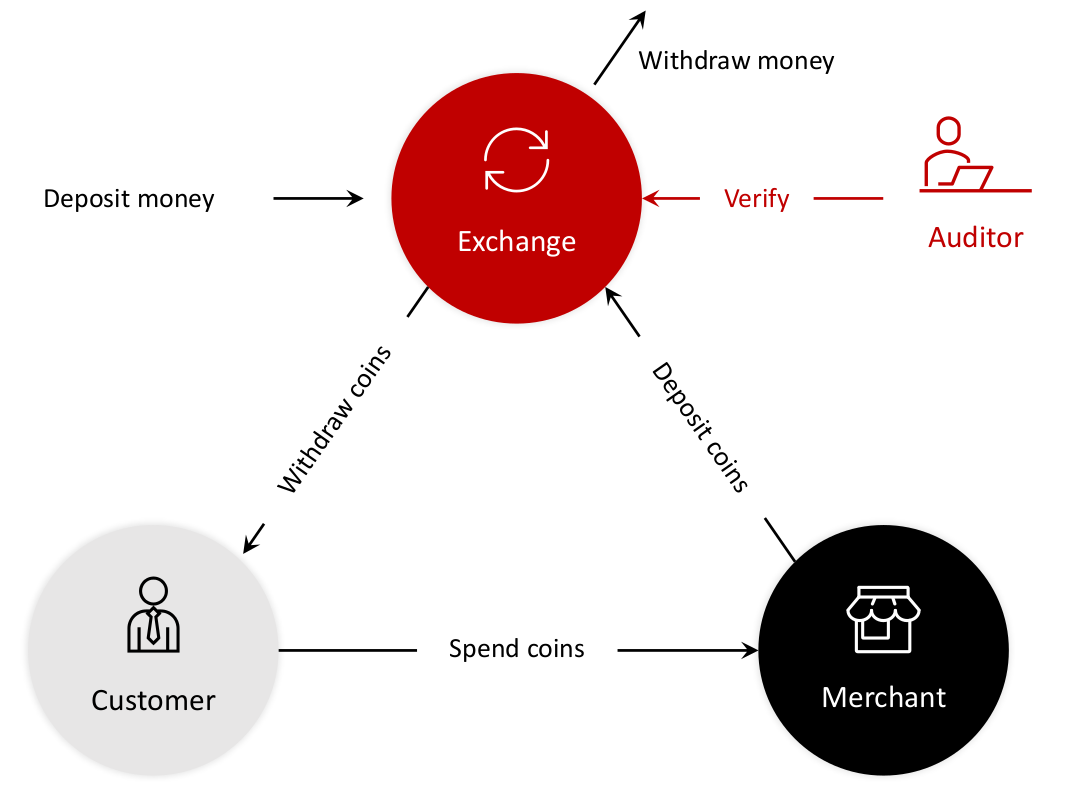
\includegraphics[height=0.6\textwidth]{diagram-simple.png}
    \centering
    \caption{GNU Taler simple overview (source: \cite{pic:simple-diagram})}
    \label{fig:simple-diagram}
\end{figure}

\subsubsection{Exchange}
\label{sec:exchange}
The exchange is the payment service provider for financial transactions between a customer and merchant.
The exchange holds bank money as reserve for the anonymous digital coins.
\\
Details of the exchange's functionality can be found in section 4.3 from Florian Dold's thesis \cite{dold:the-gnu-taler-system} or in the documentation \cite{taler-documentation:exchange-operator-manual}.
\\The code can be found in the exchange's git repository \cite{taler-git:exchange}.

\subsubsection{Customer (Wallet)}
A customer holds Taler Coins in his electronic wallet.
As we see in figure \ref{fig:simple-diagram}, a customer can withdraw coins from the exchange.
These coins can then be spent with a merchant.
\\
Details of the wallet's functionality can be found in section 4.6 from Florian Dold's thesis \cite{dold:the-gnu-taler-system} or in the documentations \cite{taler-documentation:wallet-developer-manual} \cite{taler-documentation:wallet-cli-manual}.
\\
Git Repositories:
\begin{itemize}
    \item Main repository \cite{taler-git:wallet-core} \\
          This Repository includes the wallet-core and the implementations for the web extension and CLI.
    \item Android app \cite{taler-git:android}
    \item iOS app \cite{taler-git:ios}
\end{itemize}

\subsubsection{Merchant}
A merchant accepts Taler Coins in exchange for goods and services.
The merchant deposits these coins at the exchange and receives bank money in return.
\\
Details of the wallet's functionality can be found in section 4.5 from Florian Dold's thesis \cite{dold:the-gnu-taler-system} or in the documentations:
\begin{itemize}
    \item Operator manual \cite{taler-documentation:merchant-backend-operator-manual}
    \item Merchant API \cite{taler-documentation:merchant-api}
    \item Back-Office  \cite{taler-documentation:back-office}
    \item Point-of-Sales \cite{taler-documentation:pos-manual}
\end{itemize}

\noindent Git Repositories:
\begin{itemize}
    \item Backend: \cite{taler-git:merchant}
    \item Backoffice: \cite{taler-git:backoffice}
    \item Point-of-Sales App: \cite{taler-git:android} (part of android repo)
\end{itemize}

\noindent Merchant Frontend Repositories:
\begin{itemize}
    \item Payments with Django: \cite{taler-git:django-payments}
    \item Wordpress woocommerce plugin: \cite{taler-git:woocommerce}
    \item Saleor Frontend: \cite{taler-git:saleor}
    \item Demo Frontends: \cite{taler-git:merchant-demos}
\end{itemize}

\subsubsection{Auditor}
The auditors, which are typically run by financial regulators, have the purpose to monitor the behavior of the exchanges to assure that exchanges operate correctly.
\\
Details of the auditor's functionality can be found in section 4.4 from Florian Dold's thesis \cite{dold:the-gnu-taler-system} or in the documentation \cite{taler-documentation:auditor-operator-manual}.
\\Git Repositories:
\begin{itemize}
    \item Main repository \cite{taler-git:exchange} (Part of exchange repository, inside ./src/auditor and ./src/auditordb)
    \item Auditor's public website \cite{taler-git:auditor}
\end{itemize}

\subsubsection{Bank}
The banks receive wire transfer instructions from customers and exchanges.
As long as the banks can make wire transfers to each other, the Taler parties do not have to have the same bank.

\subsection{Taler Step by Step}
\begin{figure}[htp]
    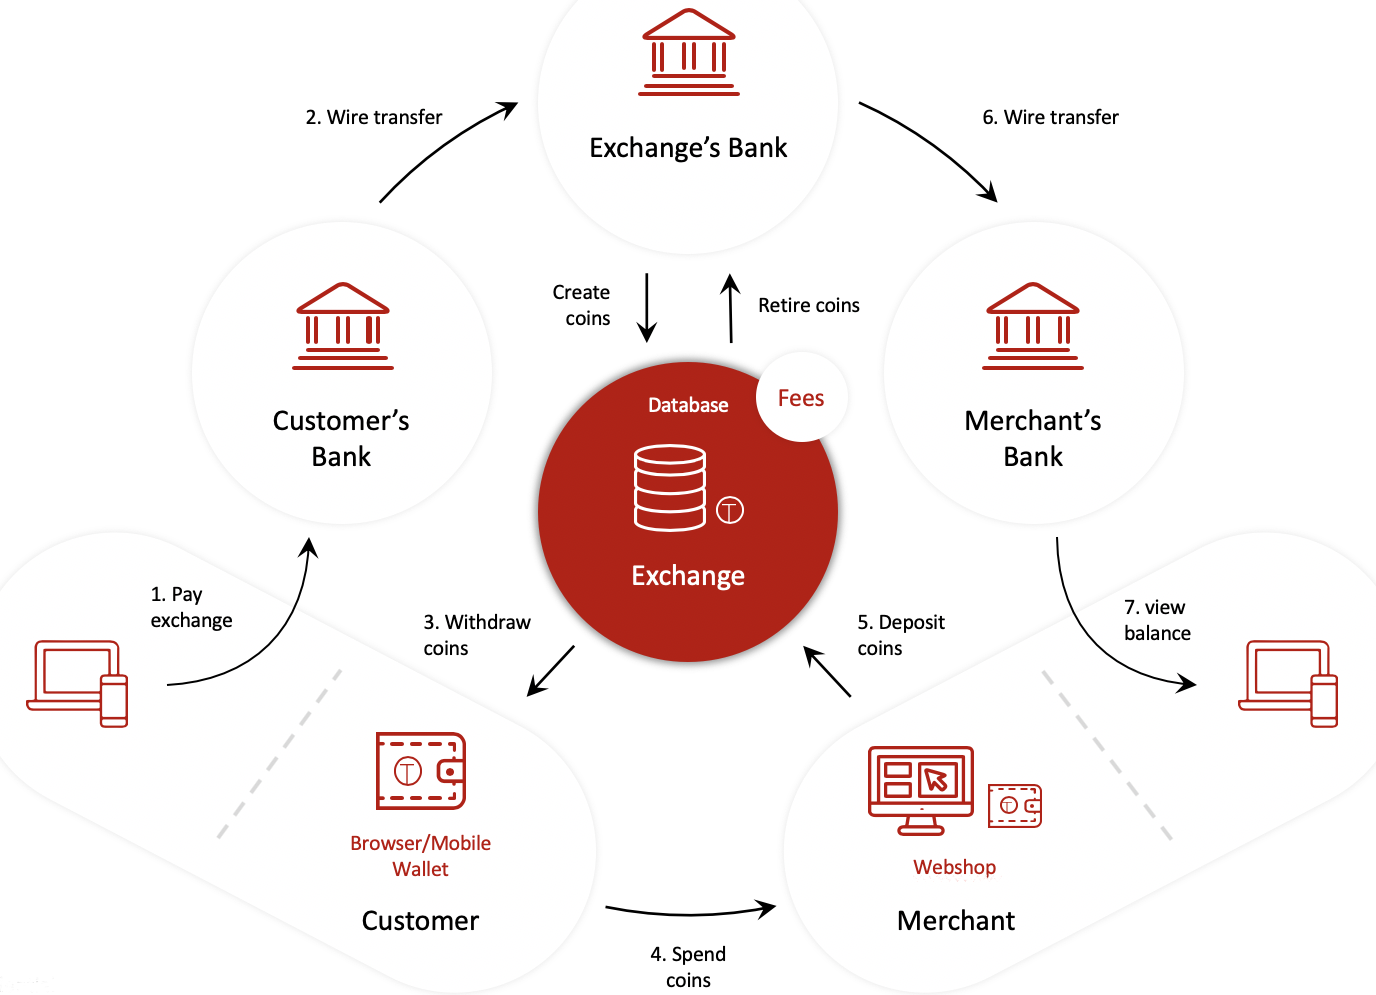
\includegraphics[height=0.65\textwidth]{taler_bigger.png}
    \centering
    \caption{GNU Taler overview (source: \cite{pic:taler-overview})}
    \label{fig:taler-overview-big}
\end{figure}
This is a high-level overview of what Taler generally does.
Many details (like privacy of the buyer, income transparency) are left out and are explained in the following sections.
We see in Figure \ref{fig:taler-overview-big} how Taler works step by step (at a high-level).
\begin{enumerate}
    \item The customer decides to withdraw Taler coins. To do this, he goes to his bank and gives the order to pay the exchange.
    \item The customers bank receives the customers order and makes a wire transfer to the exchanges Bank.
    \item The exchange has received the money and the customer can now withdraw coins to his wallet.
    \item The customer can now spend his coins at a merchant or merchants of his choice.
    \item The merchant can then deposit the coins at the exchange.
    \item The exchanges bank makes a wire transfer to the merchants bank.
    \item The merchant has successfully received the money for the goods he sold.
\end{enumerate}

\subsection{Protocols Overview}
This section provides a high-level overview of the different Taler protocols.
The details are here omitted and discussed later.

\subsubsection{Refresh Protocol}
Taler has a quite interesting protocol to get change.
The purpose of the protocol is to give unlinkable change.
When a customer buys something from a merchant, in most situations he does not have the exact sum in coins.
For this reason, change is needed to provide a convenient payment system.
A coin can be partially spent.
When this happens, the exchange and the merchant know that this coin is used for that specific contract.
If the rest of this coin would be spent in future, one could link these two transactions.
Therefore, a mechanism to get unlinkable change while still preventing money laundering or tax evasion is needed.

\subsubsection{Refund}
Taler has a built-in refund functionality.
Merchants can instruct the exchange to refund a transaction before the refund deadline.
The customer then refreshes the coin(s) in order for payments to remain unlinkable.

\subsubsection{Payment Fees}
The exchange can charge fees for withdrawal, refreshing, deposition of coins.
These fees can depend on the denomination since different denominations can have different storage requirements.
Merchants are able to cover these costs fully or partially.
\\Exchanges are also able to aggregate wire transfers to merchants, thus reducing wire transfer fees.

\subsubsection{Tipping}
Merchants can give customers a small tip.
This feature can be useful for different use cases, for example a merchant can give a tip when a customer participates in a survey.

\subsubsection{Auditing}
Financial auditing is built-in to Taler in the form of auditors.
Auditors have read access to certain exchange databases.
Their task is to verify that exchange work as expected, see chapter 4.4 in Florian Dold's thesis \cite{dold:the-gnu-taler-system} for more details.
In future versions, the auditor will provide an interface that can be used by merchants to submit deposit confirmation samples.
This can be used to detect compromised signing keys or a malicious exchange.

\subsection{Properties}
\label{sec:taler-properties}
This section describes Taler's properties.

\subsubsection{Free Software}
The core components of \acl{Taler} are under the following licenses:
\begin{itemize}
    \item exchange \cite{taler-git:exchange}: \ac{GNU AGPL}
    \item merchant \cite{taler-git:merchant}:
          \begin{itemize}
              \item backend: \ac{GNU GPL}v3+, \ac{GNU AGPL}
              \item library: \ac{GNU LGPL}
          \end{itemize}
    \item wallet-core \cite{taler-git:wallet-core}: \ac{GNU GPL}
\end{itemize}

\newpage

\subsubsection{Buyer Privacy Protection}
Taler protects the privacy of buyers during the different stages in the lifetime of a coin:
\begin{enumerate}
    \item Reserve: The reserve is identified by a key pair (private and public key).
          This means that the exchange doesn't know the identity of the reserve account holder.
          Whoever knows the private key is able to withdraw from the corresponding reserve.
    \item Withdrawal: The withdrawal process is encrypted with TLS and uses a blind signature scheme.
          Therefore the exchange doesn't know which customer holds which coin.
    \item Payment: The complete payment process doesn't rely on any information identifying a customer.
\end{enumerate}
Beware that an anonymous bi-directional channel is assumed for communication between the customer and the merchant as well as during the retrieval of denomination key from the exchange and change for partially spent coins (between customer and exchange).

\subsubsection{Merchant Taxability}
Merchant's incomes are transparent to auditors which makes taxation by the state possible.
\newline
A buyer could theoretically transfer the private key and signature of a coin directly to the merchant to bypass the exchange.
However, this is suboptimal for the merchant because the knowledge of the coin doesn't grant him the sole ownership.
If the customer spends the coin in another transaction before the merchant, the coin is voided before the merchant claims its value, thus rendering this form of payment unusable.
The same principle holds for change (refreshed coins) because it is linked to the original coin.
Whoever knows the private key and signature of the original coin can obtain the change and use it before the merchant.

\subsubsection{\acl{AML} and \acl{CFT}}
Every transaction contains the cryptographic hash of the associated contract.
This enables the authorities to request the merchant to reveal the transaction details (the contract).
If the merchant isn't able to reveal the contract, in other words fails to deliver a contract with the same hash which is included in the transaction, he risks punishment or further investigation.
\\Another aspect for \ac{AML} and \ac{CFT} are \ac{KYC} checks.
\acl{KYC} checks require certain institutions to verify certain information about their business partners in order to prevent money laundering and terrorism (see \cite{dewiki:205456999}).
\\\acl{Taler} implements these \ac{KYC} checks:
\begin{itemize}
    \item Exchanges know the identities of their customers.
    \item Merchants might need to pre-register with exchanges (depending on the deployment scenario).
\end{itemize}

\subsubsection{Payer Fraud Prevention}
The following definition was taken from the BigCommerce website \cite{website:bigcommerce-payment-fraud}.
\begin{center}
    \textit{
        "Payment fraud is any type of false or illegal transaction completed by a cybercriminal. The perpetrator deprives the victim of funds, personal property, interest or sensitive information via the internet."
    }
\end{center}
Prevention of payment fraud is a design goal for \acl{Taler}.

\subsubsection{Minimal Information Disclosure}
\acl{Taler} aims to disclose as minimal information as possible.
This mostly concerns customers, but merchants also profit by keeping financial details hidden from competitors.

\subsubsection{\acl{SPOF} Avoidance}
\ac{SPOF}s are fatal because a failure in this component can bring the complete system to a halt.

\subsubsection{Offline Payment (unsupported)}
\acl{Taler} doesn't offer offline payments due to the CAP problem (see chapter "Challenges of offline payments" in \cite{grothoff-dold:euro-bearer-online}).


\section{Cryptographic Preliminaries}
\label{sec:crypto-preliminaries}
In this section we will cover the necessary preliminaries to understand Taler.
For this part we took most of the information from Nigel P. Smarts book Cryptography made simple \cite{modernCrypto} and from the course "Applied Cryptography" at the BFH.
The chapter includes preliminaries of the already implemented cryptographic schemes and the ones that are implemented during this work.

\subsection{Hash Functions}
As source for this section, page 271-275 were used in \textit{Cryptography made Simple}  \cite{modernCrypto}.
\label{sec:hashfunc}
In this paper a hash function is always a cryptographic hash function.
Cryptographic hash function are one-way functions $H()$, which are calculating the hash value $h$ from a message $m$ so that $ h = H(m)$.
With known input one can easily calculate the hash value.
The other way around is computationally infeasible.
\\ Cryptographic hash functions have the following properties.

\subsubsection{(First) Preimage Resistance}
\label{sec:first-pre-resist}
It should be hard to find a message with a given hash value.
For a given output $y$ it is impossible to calculate the input $x$ such that $ h(x) = y$.
\\ This basically means, a hash function can not be inverted, not even with unlimited computing power.
Too much information is destroyed by the hash function and there are many values resulting in the same hash.

\subsubsection{Second Preimage Resistance}
\label{sec:second-pre-resist}
Given one message, it should be hard to find another message with the same hash value.
For a given $x_1$ and $h(x_1)$ it is hard to find a $x_2$ such that $h(x_1) = h(x_2)$.

\subsubsection{Collision Resistance}
\label{sec:col-resist}
It should be hard to find two messages with the same hash value.
It is quite obvious that collisions are existent, since there are more possible messages than hash values.
This is also known as the pigeonhole principle.
Even if there are hash collisions, it should be hard to find $x_1 \ne x_2$ such that $h(x_1) = h(x_2)$.
Due to the birthday paradoxon (a detailed description can be found under \cite{enwiki:1019272750}) it is easier to cause a collision of two arbitrary messages than of a specific message.

\subsection{Key Derivation}
\label{sec:kdf}
A \ac{KDF} derives one or more cryptographically strong secret keys from initial keying material by using a \acl{PRF}.
Therefore, input of a \ac{KDF} is some sort of keying material (e.g. from a key exchange).
Output will be a pseudo-random bit-string, which can be used as new key material.


\subsubsection{\acl{PRF}}
A \ac{PRF} is a deterministic function whose output appears to be random if the input is unknown.
The output is computationally indistinguishable from a true random source.
Different PRFs exist, for example \ac{AES} or HMAC could be used as \ac{PRF}.
In the case of \gls{hkdf}, HMAC is a suitable choice as \ac{PRF}.

\subsubsection{HMAC}
\label{sec:hmac}
A \acl{MAC} (\ac{MAC}) provides \textbf{unforgeability}, which means, only a person who knows the key $k$ can compute the MAC.
Further, a MAC protects the \textbf{message integrity}, since unauthorized changes are being detected.
Last but not least, \textbf{message authenticity} is provided too, since only a person who knows the key can compute the HMAC.
However, it does not provide non-repudation because it is a shared secret.
MACs take a message and a key as input and give the MAC tag as output.
\\One way to design such MACs is by using a hash function.
The obvious way one would design such a function would most likely be: $ t = H(k || m || pad)$
However, this variant would be \textbf{completely insecure} with hash functions based on Merkle-Damgard constructions.
Because of the structure of such hash functions, it is easy to find $H(M || X)$ for an arbitrary $X$ and a hash value $H(M)$, with that a so called \textit{length-extension} attack is possible.
\\HMAC prevents this attack by computing the MAC as follows: $t = $ HMAC$_k(m) = H( (k \oplus opad) || H( (k \oplus ipad) || m) ) $
\\ H() could be any standard hash functions, for example SHA-256, SHA-512 or SHA-3.
$\oplus$ stands for the XOR operation.
HMAC is specified in \cite{rfc2104}.

\subsubsection{HKDF}
\gls{hkdf} follows the \textit{extract-then-expand} paradigm and therefore has two phases.
In the extract phase, the input keying material is taken and a fixed-length pseudorandom key $K$ is \textit{extracted}.
This phase is used to generate a high entropy pseudorandom key from potentially weaker input keying material.
This key $K$ is used in the \textit{expand} phase to output a variable-length, pseudorandom key.

The \gls{hkdf} makes use of HMAC (\ref{sec:hmac}) instantiated with a hashfunction \ref{sec:hashfunc}.
It takes the input keying material, a salt and the length of output keying material as arguments.
\gls{hkdf} is specified in \cite{rfc5869}.

\subsection{Digital Signatures}
\label{sec:sign-schemes}
As source for this section, page 216-218 were used in \textit{Cryptography made Simple}\cite{modernCrypto}.
A digital signature is a cryptographic function used to verify the origin and integrity of a message.
It provides the following properties:
\begin{itemize}
    \item Sender authenticity: The origin/sender of a message can not be forged.
    \item Message integrity: No unauthorized change to the message can be made, the message is tamperproof.
    \item Non-repudiation: After a message is signed, one can not dispute that a message was signed.
\end{itemize}
If verification is successful, only Alice knows her private key and Bob uses Alice's public key to verify, then Bob knows that this message is really from Alice and the message has not been tampered or further modified.
A digital signature scheme has a message space M, a signature space S and three algorithms:
\begin{itemize}
    \item Key generation: $(pk,sk) \gets keyGen()$
    \item Signature generation: $s \gets $sign$_sk(m)$
    \item Verification: $ v \gets $verify$_pk(m,s)$ where $v \in {0,1}$
\end{itemize}
If the result of the verification algorithm equals 1, a signature for m is called valid.
\\Digital signatures are publicly verifiable, which means anyone can verify that $(m,s)$ is legitimate.

\subsubsection{Adversary Models \& Provable Security}
\label{sec:euf-cma}
Digital Signature schemes are believed to be secure when they are EUF-CMA secure.
\acl{EUF} (\ac{EUF}) means that given a public key $pk$ the adversary cannot construct a message with a valid signature, except with a negligible probability.
\acl{CMA} (\ac{CMA}) means that an adversary can ask a signing oracle to produce valid signatures $s' = sign_{sk}(m')$ for arbitrary messages $m' \ne m$.\\
EUF-CMA is therefore existentially unforgeability under chosen message attack and is a standard security model for digital signatures.
More details can be found in page 217-218 in \textit{Cryptography made Simple} \cite{modernCrypto}.


\subsubsection{RSA-FDH Signature Scheme}
As source for this section, pages 300-301 and 333-335 were used in \textit{Cryptography made Simple} \cite{modernCrypto}.

\label{sec:rsa-fdh}
RSA-FDH is a deterministic digital signature scheme which provides authenticity, message integrity and non-repudation.
The RSA signature scheme (without the full domain hash) is NOT \ac{EUF} secure and is vulnerable to existential forgery attacks.
RSA-FDH is one possible solution for a EUF-CMA secure scheme. EUF-CMA and its adversary model is further discussed in section \ref{sec:euf-cma}.
RSA-FDH is EUF-CMA secure under factoring and RSA assumptions.
More details on the hardness assumptions can be found on page 32-49 in \textit{Cryptography made Simple} \cite{modernCrypto}.

\paragraph{\acl{FDH}}
A \acl{FDH} is a hash function with an \textbf{image size equal to the size of the RSA modulus}.
The hashfunction $h()$ used in the RSA-FDH sign (section \ref{sec:rsa-fdh-sign}) and RSA-FDH verify (section \ref{sec:rsa-fdh-sign}) needs to fulfill all the security properties we defined in chapter \ref{sec:hashfunc}.
This means that the image is a co-domain of the RSA group $\mathbb{Z}_N^*$.
Provided that the hashfunction has properties of a random oracle, \textbf{RSA-FDH is provably EUF-CMA secure} under the RSA assumption.

\paragraph{RSA Key Generation}
\label{sec:rsa-keygen}
The information in this section is from the script of the BFH module \textit{Public Key Cryptography} taught by Prof. Dr. Walter Businger (\cite{businger:public-key-crytpo}).
The RSA private and public key are generated like this:
\begin{enumerate}
    \item Generate two random prime numbers $ p, q $ where $ p \neq q $
    \item Calculate $ N = pq $
    \item Calculate $ \lambda = \text{lcm}(p-1, q-1) $
    \item Randomly choose a number $ d $ which is bigger than $ p $ and $ q $ and where $ \text{gcd}(d, \lambda) = 1 $
    \item Calculate $ e $, the multiplicative inverse of $ d \mod \lambda $
    \item The public key is $ (e, N) $, the private key is $ (d, N) $
    \item Destroy all numbers not included in the private or public key
\end{enumerate}
Note that "lcm" stands for least common multiplier and "gcd" means greatest common divisor.
The original RSA specification uses $ \phi(n) = (p-1)(q-1) $ instead of $ \lambda = \text{lcm}(p-1, q-1) $.
$ \phi(n) $ is a multiple of $ \lambda $ (for details see \cite{businger:public-key-crytpo}).

\paragraph{Signature Algorithm}
\label{sec:rsa-fdh-sign}
The signature can be calculated as following:
\\ $ s \gets (\text{FDH}(m))^d \mod N$

\paragraph{Verification Algorithm}
\label{sec:rsa-fdh-verify}
The signature can be validated as following:
\\ $ \text{FDH}(m) \gets s^e \mod N$

\subsubsection{Schnorr Signature Scheme}
\label{sec:schnorr-sig}
The Schnorr Signature scheme is a randomized signature scheme, which is proven to be EUF-CMA secure under \ac{DLP}.
More information about the \ac{DLP} can be found in chapter 3 of \textit{Cryptography made Simple} \cite{modernCrypto}.
In february 2008 the patent expired and Schnorr signatures are now becoming widely deployed. (eg. EdDSA).
Schnorr signatures gained quite some attraction lately, since Bitcoin has announced to support Schnorr signatures starting from Block 709632 (see \cite{bip:schnorr-bitc}, \cite{btc:releasnotes-0.21}, and \cite{git:secp256k1-schnorr}).
As reference for the Schnorr signature scheme (and later Clause Blind Schnorr Signature Scheme) we use the paper \textit{Blind Schnorr Signatures and Signed ElGamal Encryption in the Algebraic Group Model} \cite{cryptoeprint:2019:877} as general source for Schnorr related schemes.

\paragraph{Setup}
We have a Group $\mathbb{G}$ of order $p$ and a generator $G$ of the group.
Further a Hashfunction $H: \{0,1\}* \rightarrow \mathbb{Z}_p$ is used.

\paragraph{Key Generation}
The key generation is the same as in \ac{DSA}.
\begin{enumerate}
    \item private key is a random integer $x \leftarrow random \in \mathbb{Z}_p$
    \item public key is $X \leftarrow xG$
\end{enumerate}

\paragraph{Sign}
The sign function takes the secret key $x$ and the message $m$ to be signed as argument.
The interactive version with a signer and a user can be seen in figure \ref{fig:schnorr-sign-protocol}.
\begin{enumerate}
    \item choose $r \leftarrow random \in \mathbb{Z}_p $
    \item calculate $R := rG$
    \item $ c := H(R,m)$
    \item $s := r + cx \mod p$
    \item $\sigma := (R,s)$
    \item return $\sigma$
\end{enumerate}

\begin{figure}
    \begin{equation*}
        \begin{array}{ l c l }
            % preliminaries
            \text{User} &  & \text{Signer}
            \\ \text{knows:} & \text{public parameters:} & \text{knows:}
            \\ \text{public key } X & \langle p, \mathbb{G}, G, H\rangle & \text{private signing key } x, X := xG
            \\ & & n \leftarrow random \in \mathbb{Z}_p
            \\ & & R := nG
            \\ & \xleftarrow[\rule{2.5cm}{0pt}]{R} &
            \\ c := H(R,m)
            \\ & \xrightarrow[\rule{2.5cm}{0pt}]{c} &
            \\ & & s := n+cx \mod p
            \\ & \xleftarrow[\rule{2.5cm}{0pt}]{s} &
            \\ \text{check } sG = R + cX
            \\ \sigma := \langle R,s \rangle
        \end{array}
    \end{equation*}
    \caption{Schnorr signature protocol with user who wants to sign a message $m$ by the signer}
    \label{fig:schnorr-sign-protocol}
\end{figure}


\paragraph{Verify}
The verify function takes the public key $X$, the message $m$ and the signature $\sigma$ as argument.
\begin{enumerate}
    \item $ c := H(R,m)$
    \item check $sG = R + cX$
    \item return true if check was successful, false otherwise
\end{enumerate}

The verification holds because $sG = R + cX  $ is $ (r + cx)G = rG + cxG$ which is equal.

\subsubsection{\acl{EdDSA}}
\ac{EdDSA} is a scheme for digital signatures based on twisted Edwards curves and the Schnorr signature scheme.
The information described here originates from \cite{rfc8032} and \cite{enwiki:1013094030}.
\ac{EdDSA} is a general algorithm that can be used with different curves. A choice in curves consists of 11 parameters. These are the most important (the others can be found in \cite{rfc8032}:
\begin{itemize}
    \item odd prime power q (used to generate elliptic curve over finite field $ \mathbb{F}_q $)
    \item integer b, where $ 2^{b-1} > q $, describing the bit size of various elements
    \item cryptographic hash function $ H $ with output size of $ 2b $
    \item base point on curve $ B $ (generator)
    \item number $ c $, (either 2 or 3)
    \item prime number L where $ LB = 0 $ and $2^c*L = \text{number of points on the curve} $
\end{itemize}

\paragraph{Key Creation}
\label{sec:eddsa-keygen}
The private key $ k $ is a random bit-string of length $ b $.
The public key $ A $ is a point on the curve.
To generate it, we calculate $ A = sB $ where $ s = H(k)[:b] $ (meaning that we take the $ b $ least significant bits from the output of the hash function as $ s $).

\paragraph{Signature Creation}
\label{sec:eddsa-signature-creation}
An \ac{EdDSA} signature of a message $ M $ is composed of $ (R, S )$, which are generated as follows:
\begin{align*}
    s & = H(k)[:b]
    \\r &= H(H(k)[b + 1:2b] \text{ || } M )
    \\R &= rB
    \\S &= (r + H(R || A || M) * s) \mod L
\end{align*}
Note that $ [:b] $ means taking the $ b $ least significant bits, $ [b + 1:2b] $ means taking the b most significant bits and $ R || A $ means concatenating $ R $ and $ A $.

\paragraph{Signature Verification}
$ (R, S) $ is the signature, $ M $ is the message, $ A $ is the public key and $c, B $ are curve parameters.
To verify a signature, the following equation must be satisfied:
\\$ 2^cSB = 2^cR + 2^cA*H(R || A || M) $
\\This means that verify() returns 1 if the equation holds and 0 otherwise.

\paragraph{Ed25519}
\label{par:curve25519}
Ed25519 is an \ac{EdDSA} based signature scheme and uses \gls{25519} (see \cite{bern:curve25519}), which offers 128 security bits.
\gls{25519} gets its name from the prime $ 2^{255} - 19 $ and is designed for fast computation and to resist side channel attacks.
\\These are the most important \ac{EdDSA} parameters for Ed25519 (the others can be found in \cite{rfc8032}):
\begin{itemize}
    \item $ q = 2^{255} - 19 $
    \item $ b = 256 $
    \item $ H() $: SHA-512
    \item $ B = (15112221349535400772501151409588531511454012693041857206046113283949847762202, $
          \\ $46316835694926478169428394003475163141307993866256225615783033603165251855960) $
    \item $ c = 3 $
    \item $ L = 2^{252} + 27742317777372353535851937790883648493 $
\end{itemize}
\subsection{Blind Signature Schemes}
\label{sec:blind-sign-schemes}
\label{sec:blind-sign-perfect-blindness}
One could think of blind signatures as a message put into an envelope made of carbon paper. The signer stamps his signature on the envelope and due to the properties of a carbon paper, the message is now signed too. (the stamp "stamps" through the envelope on the message).
The client then can open the envelope, and he possesses a correctly signed message.
This is achieved by the client by blinding the message with a blinding factor before sending to the signer ("blind()" operation).
The signer signs the blinded message and returns the signature of the blinded message to the client.
The client, who possesses the blinding factor can then unblind the signature and gets a signature of the original message ("unblind()" operation).
The explanation above leads us to the additional security property of a blind signature, the \textit{blindness} of signatures.
This property requires that a signer cannot link a message/signature pair to a particular execution of the signing protocol \cite{cryptoeprint:2019:877}.\\
A blind signature scheme is called \textit{perfectly blind} if the generated signature (\textit{unblinded} signature) is statistically independent of the interaction with the signer (\textit{blinded} signature).
Thus, blind signatures cannot be linked to the signer interaction in an information theoretic sense. \cite{schnorr:perfect-dl-signatures} \cite{spring:wallet-db-with-observers}
\subsubsection{RSA Blind Signature Scheme}
\label{sec:blind-rsa-sign}
As source for this section, the course material from "Applied Cryptography" from BFH and \cite{chaum:blind-sign} were used.
The process for receiving a valid signature from the exchange uses a blind signature scheme invented by David Chaum (\cite{chaum:blind-sign}) which is based on RSA signatures.
The process is described in figure \ref{fig:blind-sign}.
\\Note that Bob (the signer) uses a standard RSA signature and can't verify if the message from Alice is blinded.
\begin{figure}[htp]
    \begin{equation*}
        \begin{array}{ l c l }
            \text{Alice} &  & \text{Bob}
            \\ \text{knows:} & & \text{knows:}
            \\ \text{RSA public key } D_B = e, N & & \text{RSA keys } d_B, D_B
            \\ \text{message } m & &
            \\ & &
            \\ \text{blind:} & &
            \\ r \leftarrow random \in \mathbb{Z}_N^* & &
            \\ m' = m*r^{e} \mod N & &
            \\ & \xrightarrow[\rule{2.5cm}{0pt}]{m'} &
            \\ & & \text{sign:}
            \\ & & s' = (m')^{d_B} \mod N
            \\ & \xleftarrow[\rule{2.5cm}{0pt}]{s'} &
            \\ \text{unblind:}& &
            \\ s = s'*r^{-1} & &
        \end{array}
    \end{equation*}
    \caption{Blind signature scheme}
    \label{fig:blind-sign}
\end{figure}
Mathematically a blind signature works similar to the "naive" RSA signature scheme.
We consider Alice as the party who wants to have a message $m$ blindly signed by Bob.
Bob has a public key $D_B = (e, N)$ and his corresponding private key $d_B$ known only by Bob.
Alice needs to generate a random blinding factor $r\in \mathbb{Z}_N^*$, which needs to remain secret.
Alice then calculates $m'=m*r^e \mod N$. The blinded value $m'$ will now be sent to Bob by Alice.
Bob on his side calculates now the signature as usual: $s' = m'^{d_B} \mod N$.
The signature $s' $ is sent to Alice by Bob. Alice can calculate the signature as following: \\$s = s' * r^{-1}$.
\\$s$ is a valid signature of $m$, while the signer, Bob, does not know $m$ nor $b$.
\\We now want to analyze this closer to understand why blind signatures work.
Let's look at this equation:
\\$ s' = m'^{d_B} = (m*r^e)^{d_B} = m^{d_B} * (r^e)^{d_B}$.
\\The interesting part for now is $(r^e)^{d_B}$, since this is $r^1$.
This means the signature $s'$ we got from Bob is $s' = m^{d_B} * r^1$.
Now it is quite obvious how the valid signature $s$ can be calculated by multiplying with the inverse of $r$ as in: $ s =  m^{d_B} * r^1 * r^{-1} = s' * r^{-1}$.

\paragraph{Blindness}
\label{par:prop-blindness-rsa}
\gls{RSABS} are considered \textit{perfectly blind} (see \autoref{sec:blind-rsa-sign}).
There exist multiple $\langle r, m \rangle$ pairs that matches $m'$ such that $m' = m * r^e \mod N$.
Thus, \gls{RSABS} achieves \textit{perfect blindness} which cannot be attacked by brute-force or similar attacks.
Even if a valid $\langle r, m \rangle$ pair is found, the attacker has no possibility to know if it is the correct pair without additional information.

\paragraph{RSA Blinding Attack}
There are also some possible attacks on this scheme.
First this is subject to the RSA blinding attack.
In this attack the property is used, that the signing operation is mathematically equivalent to the encrypt operation in RSA.
The attacker has a ciphertext $c = m^d$ and he wants to break this message.
Now, the attacker uses the ciphertext $c$ as "message" in the blind signature scheme above.
\\$m'' = cr^e \mod n = (m^e \mod n) * r^e \mod n = (mr)^e \mod n$.
    \\The Attacker then sends the blinded message $m''$ to the signer who blindly signs the blinded message.
    \\$s' = m''^d \mod n = (mr)^{ed} \mod n = m*r \mod n$.
\\The attacker recovers the message now with $m = s'*r^{-1} \mod n$.
\\This attack could be prevented by the use of a padding scheme, however this would break RSA symmetry.
In blind signatures the RSA symmetry is needed, otherwise it would produce an incorrect value in the unblind operation.
\\Due to this issue; One should never use the same key for signing and encryption!
A version of blind signatures, RSA-FDH will be discussed, which solves this issue. \cite{enwiki:blind-sign}

\paragraph{Low Encryption Exponent Attack}
For this attack a possibly small message $m$ and a small public key $e$ is given.
If now $c = m^e < n$, one could compute $ m = \sqrt[e]{c} $.
Similar to the RSA blinding attack, padding could solve the issue, however RSA symmetry is needed.
To overcome this issue, RSA-FDH blind signatures are introduced in the next chapter.

\subsubsection{RSA-FDH Blind Signatures}
As source for this section, the course material from "Applied Cryptograhy" from BFH and \cite{chaum:blind-sign} were used.
\label{sec:blind-sign-fdh}
Blind signatures are discussed in \ref{sec:blind-sign-schemes}.
This version is quite similar to the blind signatures already introduced in figure \ref{fig:blind-sign}.
In addition, the \gls{fdh} introduced in section \ref{sec:rsa-fdh} is used.
The difference is that the message does not get directly blinded, it gets hashed before with a \acl{FDH}.
\\Given Alice's message $m$ and Bobs public key $D_B = (e,n)$.
As in the simple \gls{RSABS}, a random blinding factor $r\in \mathbb{Z}_N^*$ is generated.
Before the message is blinded, the \acl{FDH} $ f = \text{FDH}(m)$ is calculated, which then is blinded as in $f' = fr^e \mod n$.
Since the hash function is a \acl{FDH}, $f$ is in the RSA domain $\mathbb{Z}_N^*$.
Now proceed as in the blind signature scheme introduced in the previous section.
The blinded hash $f'$ will be transmitted to Bob who then computes the signature $s' = f'^d \mod n$ and sends $s'$ back.
Alice unblinds $s'$ and gets the valid signature $s = s'r^{-1} \mod n$.

\begin{figure}[htptp]
    \begin{equation*}
        \begin{array}{ l c l }
            \text{Alice} &  & \text{Bob}
            \\ \text{knows:} & & \text{knows:}
            \\ \text{RSA public key } D_B = e, N & & \text{RSA keys } d_B, D_B
            \\ \text{message } m & &
            \\ & &
            \\ Compute f = FDH(m) & &
            \\ & &
            \\ \text{blind:} & &
            \\ r \leftarrow random \in \mathbb{Z}_N^* & &
            \\ f' = f*r^{e} \mod N & &
            \\ & \xrightarrow[\rule{2.5cm}{0pt}]{f'} &
            \\ & & \text{sign:}
            \\ & & s' = (f')^{d_B} \mod N
            \\ & \xleftarrow[\rule{2.5cm}{0pt}]{s'} &
            \\ \text{unblind:}& &
            \\ s = s'*r^{-1} & &
        \end{array}
    \end{equation*}
    \caption{RSA-FDH blind signatues}
    \label{fig:rsa-fdh-blind-sign}
\end{figure}

This version of blind signature is not subject to the attacks introduced in the previous section.

\subsubsection{Blind Schnorr Signature Scheme}
\label{sec:blind-schnorr-sig}
The Blind Schnorr Signature Scheme \textbf{is considered broken} and should not be implemented.
This section is here to explain how blind Schnorr signatures generally work and should help to understand The Clause Blind Schnorr Signature Scheme \ref{sec:clause-blind-schnorr-sig}.

For the signer the calculations are the same as in the original Schnorr Signature Scheme \ref{fig:schnorr-sign-protocol}.
The exchange chooses a random $n \leftarrow random \in \mathbb{Z}_p$ and calculates $R := nG$ as before.
In comparison to the Schnorr Signature Scheme (see section \ref{sec:schnorr-sig}) we generate two random blinding factors $\alpha, \beta \leftarrow random \in \mathbb{Z}_p$ to achieve \textit{blindness}.
The User then calculates $R' := R + \alpha G + \beta X$.
This $R'$ is then used to calculate $c' := H(R',m)$ and is blinded with $b$ as in $c := c' + \beta \mod p$.
The challenge $c$ is then blindly signed by the signer $s := n+cx \mod p$.
The User checks if the signature is valid the same way as in the original protocol.
Finally the user has to unblind $s$ as in $s' := s + \alpha \mod p$.
Now the unblinded signature is $\sigma := \langle R',s' \rangle$.
This scheme is described in figure \ref{fig:schnorr-blind-sign-scheme}.
More details can be found in the \textit{Blind Schnorr Signatures and Signed ElGamal Encryption in the Algebraic Group Model} paper \cite{cryptoeprint:2019:877}.

%The unblinded signature can be verified with $s'G = R' + c'X$, since following equation is satisfied:\\
%$s'G = sG + \alpha G = (r + cx)G + \alpha G = R + \alpha G + \beta X + (-\beta + c)X = R' + c'X = R' + H(R',m)X$ \cite{cryptoeprint:2019:877}.\\

To verify the signature, the verifier has to check if the following equation holds:
\begin{align*}
    s'G & = R' + c' X
    \\ &= R' + H(R', m) X
\end{align*}
$ s', R' $ together form the signature, $ X $ is the public key and $ m $ is message.

The reason why this works is that the original Schnorr signature verification algorithm remains the same in blind signatures.
\begin{align*}
    sG = R + c X
\end{align*}

By replacing $ s, R, c, $ with the values used in the blind signature scheme (as in figure \ref{fig:schnorr-blind-sign-scheme})
\begin{align*}
    \\ s &= s' - \alpha
    \\ R &= R' - \alpha G - \beta X
    \\ c &= c' + \beta
\end{align*}

we receive the following equation:
\begin{align*}
    sG & = R + c X
    \\ (s' - \alpha)G &= R' - \alpha G - \beta X + (c' + \beta)X
    \\ s'G - \alpha G &= R' - \alpha G + c' X
    \\ s'G &= R' + c' X
\end{align*}

\begin{figure}[htp]
    \begin{equation*}
        \begin{array}{ l c l }
            % preliminaries
            \text{User} &  & \text{Signer}
            \\ \text{knows:} & \text{public parameters:} & \text{knows:}
            \\ \text{public key } X & \langle p, \mathbb{G}, G, H\rangle & \text{private signing key } x, X := xG
            \\ & & r \leftarrow random \in \mathbb{Z}_p
            \\ & & R := rG
            \\ & \xleftarrow[\rule{2.5cm}{0pt}]{R} &
            \\ \alpha, \beta \leftarrow random \in \mathbb{Z}_p
            \\ R' := R + \alpha G + \beta X
            \\ c' := H(R',m)
            \\ c := c' + \beta \mod p
            \\ & \xrightarrow[\rule{2.5cm}{0pt}]{c} &
            \\ & & s := r+cx \mod p
            \\ & \xleftarrow[\rule{2.5cm}{0pt}]{s} &
            \\ \text{check } sG = R + cX
            \\ s' := s + \alpha \mod p
            \\ \sigma := \langle R',s' \rangle
        \end{array}
    \end{equation*}
    \caption{The broken Schnorr Blind Signature Scheme}
    \label{fig:schnorr-blind-sign-scheme}
\end{figure}

\paragraph{Blindness}
Blind Schnorr Signatures also achieve \textit{perfect blindness} (\autoref{sec:blind-sign-perfect-blindness}). \cite{spring:wallet-db-with-observers} \cite{cryptoeprint:2019:877}

\paragraph{ROS Problem}
\label{par:ros-problem}
The security of Blind Schnorr Signatures relies on an additional hardness assumption, the \textit{\acl{ROS}} or ROS problem. \cite{Schnorr01securityof}
Solving the \ac{ROS} problem breaks the unforgeability property of blind Schnorr signatures by finding $l + 1$ signatures out of $l$ signing operations.
David Wagner showed in his paper that the \ac{ROS} problem can be reduced to the $(l+1)$-sum problem and therefore showed that an attack is practicable. \cite{wagner:generalized-bday-prob}
More details about \ac{ROS} and Wagner's algorithm can also be found in the paper \textit{Blind Schnorr Signatures and Signed ElGamal Encryption in the Algebraic Group Model} \cite{cryptoeprint:2019:877}.
\\
Due to the possible attack, Blind Schnorr Signatures are considered \textbf{broken} and should not be used.
The next section \ref{sec:clause-blind-schnorr-sig} introduces a modified version for which the \ac{ROS} problem is much harder to solve.
\\
The \ac{ROS} problem is a recent research topic.
Recently a paper about the (in)security of \ac{ROS} was published. \cite{cryptoeprint:2020:945}
The scheme introduced in the next section \ref{sec:clause-blind-schnorr-sig} is considered secure in 2021.
It is important to keep in mind that the \ac{ROS} problem is much newer and there is open research done.

\subsubsection{Clause Blind Schnorr Signature Scheme}
\label{sec:clause-blind-schnorr-sig}
The Clause Blind Schnorr Signature Scheme is a modification of the Blind Schnorr Signature Scheme for which the \ac{ROS} problem is harder to solve.
The Clause Blind Schnorr Signature Scheme does this by choosing two random values $r_0, r_1$ and calculating $R_0 := r_0G; R_1 := r_1G$.
The user generates the blinding factors twice $\alpha_0, \alpha_1, \beta_0, \beta_1 \leftarrow random \in \mathbb{Z}_p$.
The user then calculates the challenges as before $c_0' := H(R_0',m); c_0 := c_0' + \beta_0 \mod p$ and $c_1' := H(R_1',m); c_1 := c_1' + \beta_1 \mod p$.
After the signer receives the two challenges $c_0$ and $c_1$, the signer randomly chooses $b \leftarrow random \{0, 1\}$ and calculates only $s_b$ as in $s := r_b+c_bx \mod p$.
The User receives $s, b$ and can unblind the signature to receive his signature $\sigma := \langle R'_b, s'_b \rangle$.
The verification algorithm remains the same for Clause Blind Schnorr Signature Scheme.
Figure \ref{fig:clause-blind-schnorr-sign-scheme} shows the Clause Blind Schnorr Signature Scheme.
More details about the scheme can be found in the paper \textit{Blind Schnorr Signatures and Signed ElGamal Encryption in the Algebraic Group Model} \cite{cryptoeprint:2019:877}.


\begin{figure}
    \begin{equation*}
        \begin{array}{ l c l }
            % preliminaries
            \text{User} &  & \text{Signer}
            \\ \text{knows:} & \text{public parameters:} & \text{knows:}
            \\ \text{public key } X & \langle p, \mathbb{G}, G, H\rangle & \text{private signing key } x, X := xG
            \\ & & r_0, r_1 \leftarrow random \in \mathbb{Z}_p
            \\ & & R_0 := r_0G
            \\ & & R_1 := r_1G
            \\ & \xleftarrow[\rule{2.5cm}{0pt}]{R_0, R_1} &
            \\ \alpha_0, \alpha_1, \beta_0, \beta_1 \leftarrow random \in \mathbb{Z}_p
            \\ R_0' := R_0 + \alpha_0 G + \beta_0 X
            \\ R_1' := R_1 + \alpha_1 G + \beta_1 X
            \\ c_0' := H(R_0',m)
            \\ c_1' := H(R_1',m)
            \\ c_0 := c_0' + \beta_0 \mod p
            \\ c_1 := c_1' + \beta_1 \mod p
            \\ & \xrightarrow[\rule{2.5cm}{0pt}]{c_0, c_1} &
            \\ & & b \leftarrow random \in \{ 0,1\}
            \\ & & s := r_b+c_bx \mod p
            \\ & \xleftarrow[\rule{2.5cm}{0pt}]{b, s} &
            \\ \text{check } sG = R + cX
            \\ s' := s + \alpha_b \mod p
            \\ \sigma := \langle R_b',s' \rangle
        \end{array}
    \end{equation*}
    \caption{The Clause Schnorr Blind Signature Scheme}
    \label{fig:clause-blind-schnorr-sign-scheme}
\end{figure}

\paragraph{Blindness}
\label{par:prop-blindness-cs}
\gls{CSBS} also achieve \textit{perfect blindness} as in Schnorr Blind Signatures (see \autoref{sec:blind-rsa-sign}). \cite{cryptoeprint:2019:877}


\subsection{Diffie Hellman Key Exchange}
As source for this section, pages 383-386 were used in \textit{Cryptography made Simple} \cite{modernCrypto}.
\label{sec:preliminaries-DHKE}
The \acl{DHKE} is a well proofed and well understood key exchange mechanism.
\ac{DHKE} relies mainly on the \acl{DLP}.
\ac{DHKE} is used for key exchange in many protocols today (e.g. TLS cipher suites).

\subsubsection{Hardness Assumptions}
\label{sec:dlp}
As already stated, the \ac{DHKE} relies on the assumption that calculating the discrete logarithm is hard.
The \ac{DLP} is in $G$, where $G$ is a finite abelian group of prime order q.
This could either be a subgroup of the multiplicative group of a finite field or the set of points on an elliptic curve over a finite field.
Given $g,h \in G$, find x such that $g^x = h$.

Further, \ac{CDH} and \ac{DDH} are important hardness assumption, which can be reduced to the \ac{DLP}.
Hardness assumptions are introduced very briefly.
In this work we believe that these well proofed and well tested hardness assumptions hold.
(See Chapter 3.1 \textit{Cryptography made Simple} \cite{modernCrypto} for more details on DH hardness assumptions.)

\subsubsection{Protocol}
Alice and Bob want to securely exchange a key with \ac{DHKE}.
Alice has a private key $a$ and a corresponding public key $A = g^a \mod p$.
Bob has a private key $b$ and a corresponding public key  $B = g^b \mod p$.
With elliptic curves, the private key is a multiplication factor for a base point $g$ (see example on page 385 \textit{Cryptography made Simple} \cite{modernCrypto}).

Alice now sends her public key $A$ to Bob.
Bob can then calculate $k = A^b \mod p = g^{ab} \mod p$ and sends his public key $B$ to Alice.
Alice can then calculate $k = B^a \mod p = g^{ab} \mod p$.
Both get the same key $k$ as result of the key exchange.
Note: This protocol on its own is not an authenticated key exchange, which means that Man-in-the-Middle attacks are possible.

A different way of looking at \ac{DHKE} is by thinking of a lock which can be unlocked by two (private) keys.
If one of the two private keys are known, one could calculate $k$ on its own.
Taler's refresh protocol (see \ref{sec:refresh-protocol}) uses \ac{DHKE} in a very interesting way.

\subsection{Cut and Choose Protocol}
\label{sec:preliminaries-cut-choose}
A good introduction to cut and choose protocols gives the Paper from Claude Crépeau (\cite{Crépeau2005} References to the important examples can be found in the paper.):
\begin{center}
    \textit{
        "A cut and choose protocol is a two-party protocol in which one party tries to convince another party that some data he sent to the former was honestly constructed according to an agreed upon method.
        Important examples of cut-and-choose protocols are interactive proofs, interactive arguments, zero-knowledge protocols, witness indistinguishable and witness hiding protocols for proving knowledge of a piece of information that is computationally hard to find.
        Such a protocol usually carries a small probability that it is successful despite the fact that the desired property is not satisfied.
        \\\dots\\
        The expression cut-and-choose was later introduced by David Chaum in analogy to a popular cake sharing problem:
        Given a complete cake to be shared among two parties distrusting of each other (for reasons of serious appetite).
        A fair way for them to share the cake is to have one of them cut the cake in two equals hares, and let the other one choose his favourite share.
        This solution guarantees that it is in the formers best interest to cut the shares as evenly as possible."
    }
\end{center}

Talers cut and choose protocol is \textit{zero knowledge}, which means that nothing about the secret is learned.
The cut and choose protocol used in Taler is explained further when the refresh protocol is discussed (see \ref{sec:refresh-protocol}).

\section{Taler Protocols}
In section \ref{sec:taler-intro} a brief overview of how \acl{Taler} works is given. All the relevant preliminaries are covered in section \ref{sec:crypto-preliminaries}.
In this section a closer look at the different protocols is taken.

\subsection{Withdrawal Protocol}
\label{sec:withdrawal}
The withdrawal protocol is described in chapter 4.7.2 of \cite{dold:the-gnu-taler-system}.
Before coins can be withdrawn, the customer generates a reserve key pair $ w_s, W_p \leftarrow Ed25519.KeyGen() $.
He then transfers a certain amount of money from his bank to the exchange's bank via wire transfer.
This payment must include the reserve public key $ W_p $.
The customer will later authorize withdrawals with a signature using his private reserve key.
%The customer can then authenticate, since he is in possession of the private reserve key.
As soon as the exchange has received the payment, the withdrawal for coins with a value $ i $ can begin (described in figure \ref{fig:withdrawal-process}).

At this stage the client knows the reserve private key and the public denomination key.
The customer can then create coins up to the amount included in the wire transfer.
The coin creation and blind signatures are described in section \ref{sec:blind-sign-fdh}.
So the client generates a planchet (an Ed25519 key pair) and blinds it.
This blinded planchet is then signed by the customers private reserve key, to prove that the customer is eligible to withdraw the coin.
The exchange who receives the blinded planchet and the signature first checks whether the signature is valid with the public reserve key sent with the wire transfer.
When successful, the exchange blindly signs the planchet, returns the signature and notes the amount withdrawn of the reserve.
The customer unblinds the signature, checks its validity and persists the coin.
The state machine of a coin can be seen in figure \ref{fig:coin:states}.

\begin{figure}[htp]
    \begin{center}
        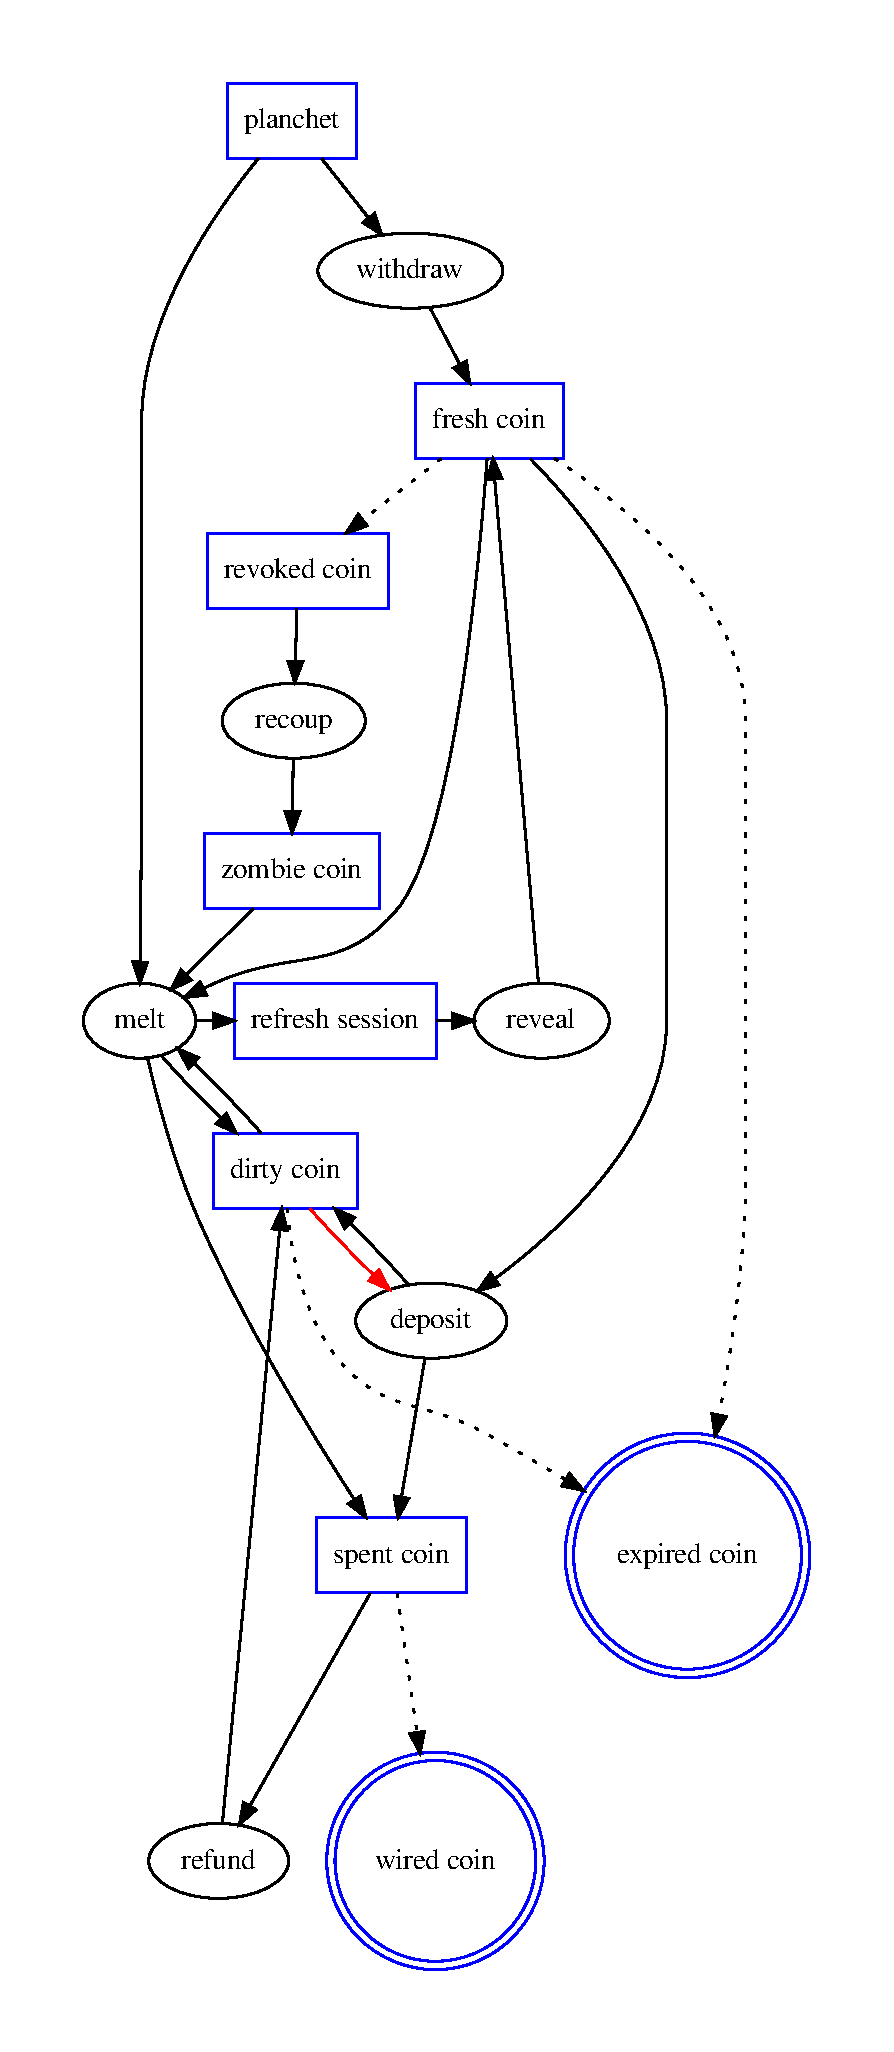
\includegraphics[scale=0.58]{coin.pdf}
    \end{center}
    \caption{State machine of a coin (source: \cite{pic:coin-state-machine})}
    \label{fig:coin:states}
\end{figure}

\begin{figure}[htp]
    \begin{equation*}
        \resizebox{1.0\textwidth}{!}{$\displaystyle
        \begin{array}{ l c l }
            \text{Customer} &  & \text{Exchange}
            \\ \text{knows:} & & \text{knows:}
            \\ \text{reserve keys } w_s, W_p & & \text{reserve public key } W_p
            \\ \text{denomination public key } D_p = e, N & & \text{denomination keys } d_s, D_p
            \\ & &
            \\\text{generate coin key pair:} & &
            \\ c_s, C_p \leftarrow Ed25519.KeyGen() & &
            \\ \text{blind:} & &
            \\ r \leftarrow random \in \mathbb{Z}_N^* & &
            \\ m' = \text{FDH}(N, C_p)*r^{e} \mod N & &
            \\ \text{sign with reserve private key:} & &
            \\ \rho_W = D_p, m' & &
            \\ \sigma_W = \text{Ed25519.Sign}(w_s, \rho_W) & &
            \\ & \xrightarrow[\rule{2.5cm}{0pt}]{\rho = W_p, \sigma_W, \rho_W} &
            \\ & & \text{verify if denomination public key}
            \\ & & \text{is valid}
            \\ & & \text{check } \text{Ed25519.Verify}(W_p, \rho_W, \sigma_W)
            \\ & & \text{decrease balance if sufficient}
            \\ & & \text{sign:}
            \\ & & \sigma'_c = (m')^{d_s} \mod N
            \\ & \xleftarrow[\rule{2.5cm}{0pt}]{\sigma'_c} &
            \\ \text{unblind:}& &
            \\ \sigma_c = \sigma'_c*r^{-1} & &
            \\ \text{verify signature:}& &
            \\ \text{check } \sigma_c^{e} = \text{FDH}(N, C_p) & &
            \\ & &
            \\ \text{resulting coin: } c_s, C_p, \sigma_c, D_p & &
        \end{array}$
        }
    \end{equation*}
    \caption{Withdrawal process}
    \label{fig:withdrawal-process}
\end{figure}

\subsubsection{Withdraw Loophole}
\label{sec:withdraw-loophole}
The withdraw loophole allows withdraw operations where owner of the resulting coins isn't the owner of the reserve that the coins where withdrawn from.
It is used for tipping (described in section \ref{sec:tipping}) and can therefore be seen as a feature.

By misusing the withdraw loophole, untaxed and untraceable payments can be performed.
Figure \ref{fig:withdraw-loophole-exploit} explains how such a payment would work.
Note that we omitted the parts leading up to the coin creation (contract, agreement of price, number of coins and their denominations).
This is how it works on a high level:
\begin{enumerate}
    \item The malicious merchant generates and blinds coins, which are then transmitted to the customer
    \item The customer authorizes the withdraw from his reserve by signing the blinded coins with the private key of his reserve, thus generating withdraw confirmations.
    \item The withdraw confirmations are transmitted to the exchange, which generates the signatures and returns them to the malicious merchant.
    \item The malicious merchant unblinds the signatures.
          He is now in possession of the coin, thus the payment is completed.
\end{enumerate}

\begin{figure}[htp]
    \begin{equation*}
        \resizebox{1.0\textwidth}{!}{$\displaystyle
        \begin{array}{ l c l}
            % preliminaries
            \textbf{Customer}          &  & \textbf{malicious Merchant}
            \\ \text{knows:} & & \text{knows:}
            \\ \text{reserve keys } w_s, W_p
            \\ \text{denomination public key } D_p = \langle e, N \rangle & & \text{denomination public key } D_p = \langle e, N \rangle
            \\
            % generate coin
            \\ & & \text{generate coin key pair:}
            \\ & & c_s, C_p \leftarrow \text{Ed25519.KeyGen}()
            % blind
            \\ & & \text{blind:}
            \\ & & r \leftarrow random \in \mathbb{Z}_N^*
            \\ & & m' := \text{FDH}(N, C_p)*r^{e} \mod N
            % sing with reserve sk
            \\ & \xleftarrow[\rule{2cm}{0pt}]{m'}
            \\ \text{sign with reserve private key:}
            \\ \rho_W := \langle D_p, m' \rangle
            \\ \sigma_W := \text{Ed25519.Sign}(w_s, \rho_W)
            \\ & \xrightarrow[\rule{2cm}{0pt}]{ \langle W_p, \sigma_W, \rho_W \rangle }
            \\
            \hline
            \\
            \textbf{malicious Merchant} &  & \textbf{Exchange}
            \\\text{knows:} & & \text{knows:}
            \\& & \text{reserve public key } W_p
            \\ \text{denomination public key } D_p = \langle e, N \rangle & & \text{denomination keys } d_s, D_p
            \\
            \\ & \xrightarrow[\rule{2cm}{0pt}]{ \langle W_p, \sigma_W, \rho_W \rangle }
            \\ & & \langle D_p, m' \rangle := \rho_W
            \\ & & \text{verify if } D_p \text{ is valid}
            \\ & & \textbf{check } \text{Ed25519.Verify}(W_p, \rho_W, \sigma_W)
            \\ & & \text{decrease balance if sufficient}
            \\ & & \text{sign:}
            \\ & & \sigma'_c := (m')^{d_s} \mod N
            \\ & \xleftarrow[\rule{2cm}{0pt}]{\sigma'_c}
            \\ \text{unblind:}
            \\ \sigma_c := \sigma'_c*r^{-1}
            \\ \text{verify signature:}
            \\ \textbf{check if } \sigma_c = \text{FDH}(N, C_p)
            \\
            \\ \text{resulting coin: } \langle c_s, C_p, \sigma_c, D_p \rangle
        \end{array}$
        }
    \end{equation*}
    \caption{Untaxed payment using the withdraw loophole}
    \label{fig:withdraw-loophole-exploit}
\end{figure}

\subsection{Payment Process}
The payment process is divided in two steps described by the spend and deposit protocols.
Details about the payment process can be found in multiple chapters in \cite{dold:the-gnu-taler-system}:
Chapter 4.7.3 describes the spend and deposit protocols.
Chapter 4.1.4 describes more general aspects as well as the contract header and deposit permission structure and details.
\\On a high level, payment works like this:
\begin{enumerate}
    \item The  customer submits a shopping cart (one or more items to buy) and commits his intent to buy them.
    \item The merchant puts together the contract terms containing the necessary information for payment, signs it and sends both to the customer (spend protocol).
    \item The customer generates a deposit permission and its signature for each coin used in the transaction (spend protocol).
    \item The customer forwards the deposit permission(s) to the merchant (spend protocol).
          If the deposit protocol is performed by the customer, this step can be skipped.
    \item Either the customer or the merchant sends the deposit permission(s) to the exchange (deposit protocol).
    \item The exchange processes the deposit permission and returns a deposition confirmation when successful (deposit protocol).
    \item If the deposit protocol was performed by the customer, the deposit confirmation(s) have to be forwarded to the merchant.
\end{enumerate}

\subsubsection{Spend Protocol}
The payment process begins when a customer submits a shopping cart (one or more items to buy) and commits his intent to buy them.
The merchant has a key pair skM, pkM of which the customer knows the public key.
Note that certain details contained in contract header or deposit permission like merchant \ac{KYC} information, deposit and refund deadlines and fees are left out.
The deposit state machine can be seen in figure \ref{fig:deposit:states}.
\begin{figure}[htp]
    \begin{center}
        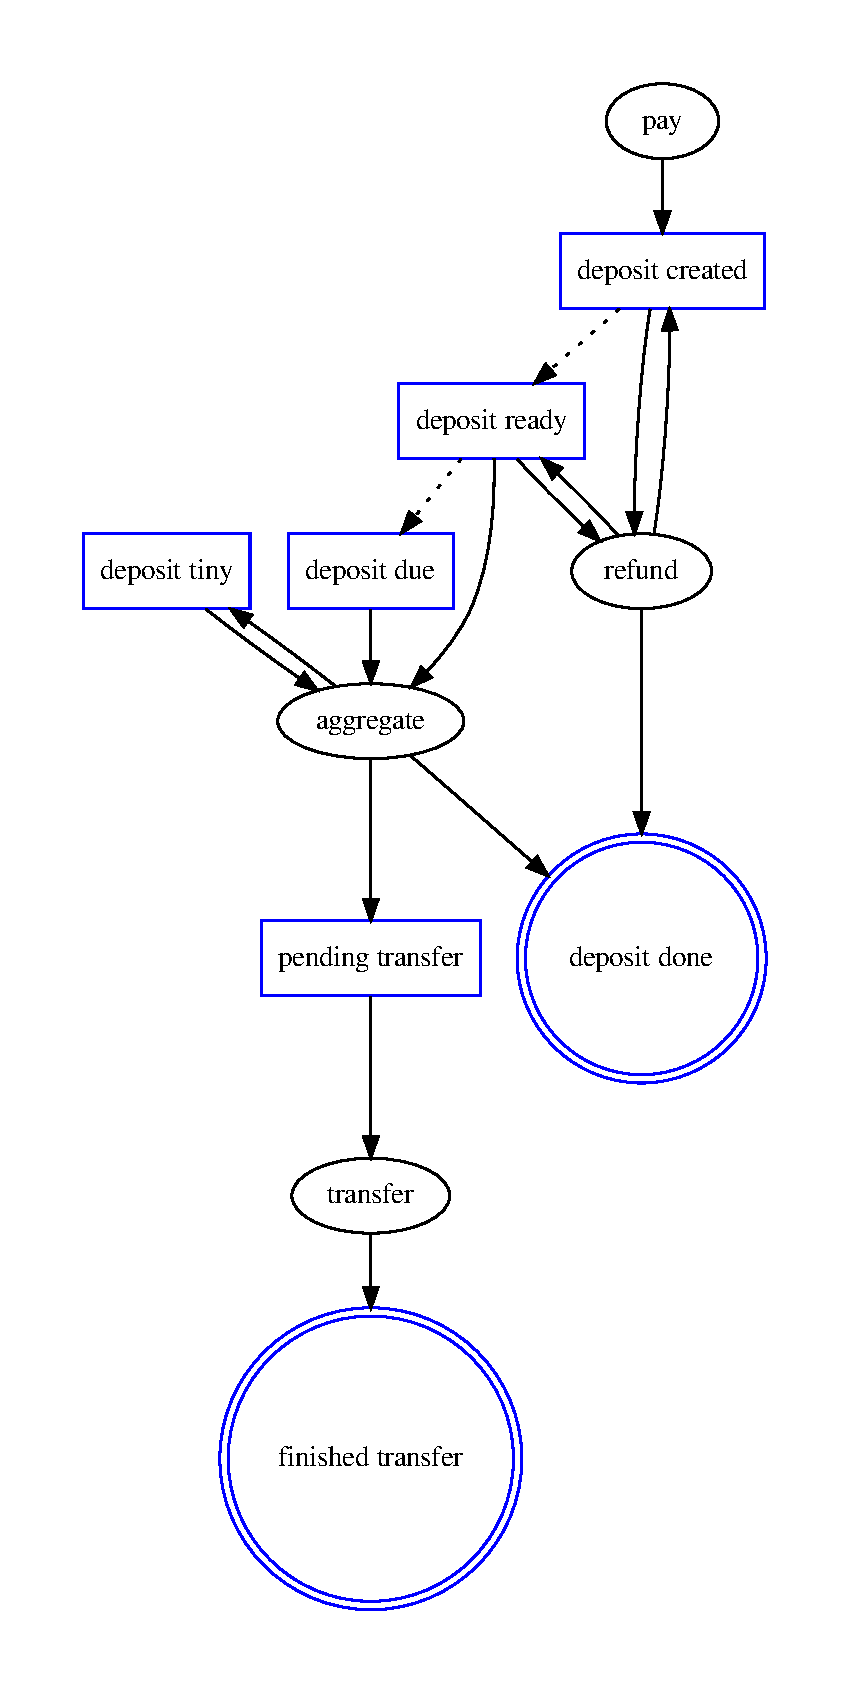
\includegraphics[scale=0.7]{deposit.pdf}
    \end{center}
    \caption{State machine of a deposit (source: \cite{pic:deposit-state-machine})}
    \label{fig:deposit:states}
\end{figure}

\begin{enumerate}
    \item The merchant puts together the following information (without transmitting them) and requests payment:
          \begin{itemize}
              \item price $ v $
              \item exchange $E_m$ (multiple possible)
              \item account $A_m$ at the exchange $E_m$
              \item info (free form details containing the full contract)
          \end{itemize}
    \item The customer generates an Ed25519 claim key pair $ p_s, P_p $ and submits the public key to the merchant.
          This key can be used by the customer to prove that he didn't copy contract terms from another customer.
    \item The merchant puts together the contract terms $ \rho  $ and signs it with skM, resulting in the signature $ \sigma_P$.
          \\The contract terms contains:
          \begin{itemize}
              \item $E_m$ (exchange)
              \item $A_m$ (account at exchange $E_m$)
              \item pkM
              \item Hash($v$, info)
              \item $ P_p $
          \end{itemize}
          $ \rho_P $ (contract terms), $ \sigma_P$ (contract terms signature), $ v $ (price) and info are submitted to the customer.
    \item The customer does the following checks:
          \begin{itemize}
              \item Is the signature of the contract terms correct?
              \item Is the public key referenced in the contract terms the same as the one generated in step 2?
              \item Is the hash of price and info the same as the one in the contract terms?
          \end{itemize}
          If all checks are successful, the customer chooses one or more coins to be spent.
          For each coin, a deposit permission $ \rho_{D} $ and its signature $ \sigma_{D} $ is generated.
          The deposit permission contains the following information:
          \begin{itemize}
              \item Coin public key $ C_p $
              \item Coin denomination public key pkD
              \item Coin signature $ \sigma_C $
              \item Value to be spent for this coin $f$ (greater than zero, up to the residual value of the coin)
              \item Hash of the contract terms $ \rho_P $
              \item Account of merchant $A_m$ (at exchange $E_m$)
              \item Merchant public key pkM
          \end{itemize}
          The list of deposit permissions and their signatures is transferred to the merchant who then executed the deposit protocol.
          Note that the customer is also able to deposit the coins (instead of the merchant), this is used in cases where the merchant doesn't have an internet connection, but the customer does.
          This can be useful in cases where the merchant becomes unresponsive.
          The customer can prove that he paid in time.
    \item The merchant receives the deposit permissions and signatures and uses the deposit protocol to execute the payment.
\end{enumerate}

Before we continue with the deposit protocol, there are a few interesting details to point out (described in \cite{dold:the-gnu-taler-system} section 4.1.4):
\begin{itemize}
    \item The contract terms and the deposit permission are \ac{JSON} objects.
    \item The contract terms only contains a cryptographic hash of the contract.
          This improves privacy since the exchange doesn't have to know the full contract details, but still makes it possible to identify the contract in case of a dispute or some form of auditing.
    \item At the point where the merchant completes step three (submits the contract terms and its signature) to the customer, the customer is able to finish the transaction using the deposit protocol without interaction of the merchant.
          This means that the merchant at this step must be able to fulfill the contract if the customer completes the payment process.
\end{itemize}

\subsubsection{Deposit Protocol}
\label{sec:deposit-protocol}
As previously mentioned, both parties (customer and merchant) are able to run the deposit protocol.
In the following description, the term merchant will be used, but could be replaced by customer.
In cases where there are multiple deposit permissions (meaning that multiple coins are used to pay), the deposit protocol is run separately for each deposit permission.
\begin{enumerate}
    \item The merchant submits the deposit permission and its signature to the exchange.
    \item The exchange runs these checks:
          \begin{itemize}
              \item Is the denomination public key referenced in the deposit permission valid (issued by the exchange, lifetime between start and deposit/refresh expiration, not revoked)?
              \item Is the deposit permission signature $ \sigma_{D} $ a correct signature of the deposit permission $ \rho_{D} $ with the Ed25519 coin public key $ C_p $ referenced in the deposit permission?
              \item Is there a processed deposit recorded in the exchanges databases based on coin public key and contract terms hash (replay/double spending)?
                    If not, continue with the next check since this is correct and expected behavior.
                    \\If there is, does the recorded deposit permission equal the one we're currently checking?
                    If this is the case, further checks can be skipped and the deposit confirmation signature can be returned to the customer.
                    If not, the process should be terminated because there's something wrong with the transaction.
              \item Is the signature of the coin valid?
              \item Is $ f $ (the value to be spent) smaller or equal the residual value of the coin (check for overspending attempt)?
          \end{itemize}
          If all checks are successful, the exchange saves the deposit record containing the deposit permission and its signature in a database, subtracts the spent value from the residual value of the coin and schedules the money transfer to the merchant's account $ A_m $ (grouping payments is done to reduce payment fees).
          \\The exchange calculates a deposit confirmation signature $ \sigma_{DC} $ for the deposit permission with the exchange signing private key and returns them to the merchant.
          \\This signature is also used to prove that a merchant was the first to receive payment from a certain coin.
          Without this, an evil exchange could later deny confirming a payment and claim double spending.
          With the signature, the merchant can prove that the payment was confirmed by the exchange, thus delegating the responsibility (and potential financial loss) for double spending detection to the exchange.
    \item The merchant checks the signatures of the deposit confirmations with the exchange signing public key.
\end{enumerate}

It may happen that a payment gets stuck as partially complete, for example when a backup of a wallet is restored and one coin or more have already been spent (\cite{dold:the-gnu-taler-system} chapter 4.1.4).
In this case, the customer can retry the payment with a different coin.
If this isn't possible, the payment can be refunded (assuming refunds were enabled for this payment).
Other scenarios were described in Dold's thesis, but dismissed due to privacy concerns.
This means that disputes have to be settled aside from Taler when a customer isn't able to fully pay and refunds are disabled.

\subsubsection{Web Payment Scenarios}
The following methods are Taler-native methods for paying and payment validation.
They are not identity-based, meaning that they do not require a login or similar techniques.
Note that other methods could be implemented depending on the scenario.

\begin{itemize}
    \item \textbf{Resource-based web payment} (\cite{dold:the-gnu-taler-system} chapter 4.1.5):
          All Taler contract terms contain a fulfillment URL.
          This can either be a direct link to a digital product (like a movie, a song or a document), or to a confirmation page.
          When a browser opens a fulfillment URL for a resource that hasn't yet been paid for, the merchant requests payment.
          The wallet then generates and submits a claim key pair, thus claiming the contract, which then can be paid (if the user accepts the contract).
          The browser can then retry to navigate to the fulfillment URL, this time submitting the contract order ID as parameter, which the merchant can check if it has been paid (and deliver the content if this is the case).
          This is known as the extended fulfillment URL
          \\The wallet stores fulfillment URLs and their associated contracts.
          Upon receiving a payment request, the wallet searches the stored fulfillment URLs and if it found one, automatically forwards the user to the extended fulfillment URL containing the contract.
    \item \textbf{Session-bound payments and sharing} (\cite{dold:the-gnu-taler-system} chapter 4.1.6):
          So far, validating payment is done using the extended fulfillment URL.
          The problem with this approach is that this URL can be shared, which is a problem for digital content.
          To make this more difficult, the seller's website assigns the user a session ID (for example using a session cookie) and extends the extended fulfillment URL with a session signature parameter.
          This parameter can be used by the merchant to check if the user paid for the resource or replayed the payment in this session.
    \item \textbf{Embedded content} (\cite{dold:the-gnu-taler-system} chapter 4.1.7):
          When paying to access multiple resources behind a paywall (instead of just one resource), the previously described methods do not work.
          Dold's thesis suggest two methods:
          \begin{enumerate}
              \item A session cookie can be set by accessing the fulfillment URL.
                    When the browser requests a subresource, the merchant can verify the session cookie.
              \item In this scenario, the fulfillment URL would show the resources behind the paywall.
                    Upon opening the extended fulfillment URL, the merchant's website would add an authentication token to the URLs of the subresources.
                    When accessing a subresource, the merchant can check the authentication tokens validity.
          \end{enumerate}
\end{itemize}

\subsection{Refresh Protocol}
\label{sec:refresh-protocol}
This section provides a description of the refresh protocol.
The technical details can be found in 4.7.4 \cite{dold:the-gnu-taler-system}.
All relevant preliminaries needed to understand the technical details were already introduced in this work.

\subsubsection{Introduction}
A protocol to refresh coins is needed for many reasons.
One important reason is giving change.
Similar to the real world, there are often situations where one does not have the exact amount of coins.
A change protocol therefore provides a lot of convenience for the users.
Without such a mechanism it would be quite hard to use. \\
Giving change is not trivial, since \ac{AML} and \ac{CFT} compliance still needs to hold.
On the other side, the change still needs to provide privacy for the customer.
Thus, the change must be unlinkable to the previous (or any) transaction.\\
Complying with \ac{AML} and \ac{CFT} while preserving the customer's anonymity may sound like a contradiction at first.
However, Taler has a clever way to solve this problem with the refresh protocol.

The general idea is that the new coin can be derived from the private key of the old coin.

\subsubsection{DH Lock}
\ac{DHKE} was introduced in section \ref{sec:preliminaries-DHKE}.
Taler uses \ac{ECDH} as a lock with two possible keys to unlock the shared key.
To create such a lock, one creates two key pairs $C = cG$ and $T = tG$.
To unlock now means calculating $k$.
Both private keys, $c$ and $t$ are now able to calculate $k = tC = t(cG) = c(tG) = cT$ and thus can unlock the lock.
This $k$ can then be used to derive the private key of the new coin and the corresponding blinding factor.

\subsubsection{Customer Setup}

The customer, which holds the old partially spend coin and knows \\$C_{old} = \text{Ed25519.GetPub}(c_{old})$.
    A transfer key $T = \text{Ed25519.GetPub}(t)$ is then (randomly) generated by the customer.
    \\The key pairs $T = \text{Ed25519.GetPub}(t)$ and $C_{old} = \text{Ed25519.GetPub}(c_{old})$ form the lock with two keys that was introduced before.
    The customer then creates $x = c_{old}, T = tC_{old}$ and derives $c_{new}$, the private key of the new coin and $b_{new}$ the blinding factor of the new key.
    As usual the customer calculates the coins public key $C_{new} = \text{Ed25519.GetPub}(c_{new})$, hashes the new coin with \gls{fdh} $f_{new} = \text{FDH}(C_{new})$ and blinds the hash $f'_{new} = f_{new}b_{new}^e$.
    The $f'_{new}$ is then transmitted to the exchange.
    \\Figure \ref{fig:refresh-derive} shows how the new coin is derived as explained above.

    \begin{figure}[htp]
        \centering
        \fbox{%
            \procedure[codesize=\small]{$\text{RefreshDerive}(s, \langle e,N\rangle, C_p)$}{%
                t := \text{HKDF}(256, s, \text{"t"}) \\
                T := \text{Curve25519.GetPub}(t) \\
                x := \textrm{ECDH-EC}(t, C_p)  \\
                r := \text{SelectSeeded}(x,\mathbb{Z}^*_N)\\
                c'_s := \text{HKDF}(256,x,"c")\\
                C'_p := \text{Ed25519.GetPub}(c'_s)\\
                \overline{m} := r^e * C'_p \mod N\\
                \pcreturn \langle t, T, x, c_s', C_p', \overline{m}\rangle
            }
        }
        \caption[RefreshDerive algorithm]{The RefreshDerive derives a new coin from a dirty coin with a seed. The DH-Lock is used to create the link used in the linking protocol}
        \label{fig:refresh-derive}
    \end{figure}

    Now with the DH Lock the person who is in possession of the old key can always recalculate and thus spend the new coin (as long as it knows the public transfer key $T$).
    However, there is one last thing: How does the exchange know that the old key is linked to the new one?
    To comply with \ac{AML} and \ac{CFT}, the exchange wants to ensure that the person who created the new coin is also in possession of the old coin.
    A link needs to be created in a way that nobody can link the old coin to the new coin, except the person in possession of the old coin.
    The person in possession of the old coin needs to proof to the exchange that this link was created without revealing the link.
    This problem is solved with the cut and choose protocol in the next section.

    \begin{figure}[htp]
        \centering
        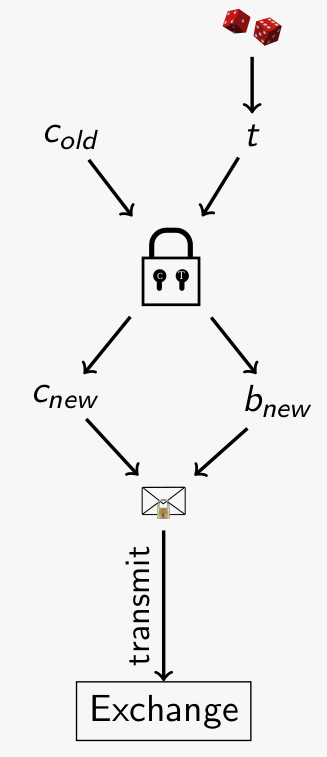
\includegraphics[height=0.5\textwidth]{taler_refresh_transfer_key.png}
        \caption{Taler refresh protocol, transfer key setup (source: \cite{pic:refresh-prot})}
        \label{fig:taler-refresh-transfer-key}
    \end{figure}
    \newpage
    \subsubsection{Cut \& Choose}
    Instead of doing the customer setup once, it is done $n$ times.
    The customer generates $n$ different transfer keys $t_1, t_2 \dots t_n$.
    For each key the whole calculations are done and all the blinded coins $f'_1, f'_2 \dots f'_n$ are sent to the exchange together with the old coins public key and signature. \\
    The exchange responds with a randomly picked number from $1$ to $n$.
    The customer has to reveal all the transfer keys, \textbf{except the one picked by the exchange.}
    The exchange makes the same calculations with the revealed private transfer keys (without knowing the private key $c_{old}$).
    The exchange can now verify whether the customer was honest or not.
    A evil customer could create a new coin which is not linked to the old coin (without the DH lock).
    Such attacks will be detected with a high probability in this protocol.
    Since the $t_x$ picked by the exchange is not checked, an evil customer can win this with a probability of $1/n$.
    Already with $n=3$ an attack is not in the customers interest due to economic reasons.
    In 2 out of 3 cases the exchange would detect the attack and would keep the money and the customer would have lost it.
    The probability can be adjusted with $n$.
    With increasing size of $n$ the attack becomes even less attractive.
    When the cut and choose protocol ended successfully, the value of the old coin is set to zero.

    \begin{figure}[htp]
        \centering
        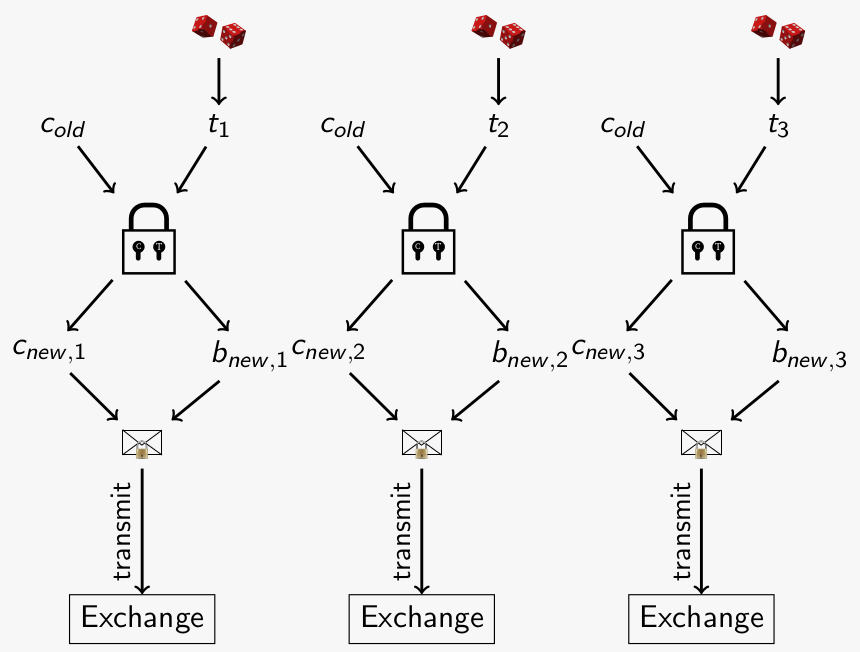
\includegraphics[height=0.5\textwidth]{taler_cut_and_choose.png}
        \caption{Taler refresh protocol, cut and choose (source: \cite{pic:refresh-prot})}
        \label{fig:taler-cut-and-choose}
    \end{figure}

    \subsection{Commit Phase}
    \label{sec:commit-phase-rsa}
    The refresh protocol is implemented in two phases.
    The commit phases creates $k$ derives and commits to this values by calculating a hash over the derives.
    On the exchange's side various checks are done to validate the request.
    Detailed steps of the commit phase are shown in figure  \ref{fig:refresh-part1}.


    \begin{figure}
        \begin{equation*}
        \resizebox{1.0\textwidth}{!}{$\displaystyle
            \begin{array}{ l c l }
                % preliminaries
                \text{Customer} &  & \text{Exchange}
                \\ \text{knows:} & & \text{knows:}
                \\ \text{denomination public key } D_{p(i)} & & \text{denomination keys } d_{s(i)}, D_{p(i)}
                \\ \text{coin}_0 = \langle D_{p(0)}, c_s^{(0)}, C_p^{(0)}, \sigma_c^{(0)} \rangle & &
                % refresh request
                \\ \text{Select} \langle N_t, e_t\rangle := D_{p(t)} \in D_{p(i)}
                \\ \textbf{for } i = 1, \dots, \kappa: % generate k derives
                \\ s_i \rightarrow \{0,1\}^{256} % seed generation
                \\ X_i := \text{RefreshDerive}(s_i, D_{p(t)}, C_p^{(0)})
                \\ (t_i, T_i, x_i, c_s^{(i)}, C_p^{(i)}, \overline{m}_i) := X_i
                \\ \textbf{endfor}
                \\ h_T := H(T_1, \dots, T_k)
                \\ h_{\overline{m}} := H(\overline{m}_1, \dots, \overline{m}_k)
                \\ h_C := H(h_t, h_{\overline{m}})
                \\ \rho_{RC} := \langle h_C, D_{p(t)}, D_{p(0)}, C_p^{(0)}, \sigma_C^{(0)}  \rangle
                \\ \sigma_{RC} := \text{Ed25519.Sign}(c_s^{(0), \rho_{RC}})
                \\ \text{Persist refresh-request} \langle \rho_{RC}, \sigma_{RC} \rangle
                \\ & \xrightarrow[\rule{2.5cm}{0pt}]{\rho_{RC}, \sigma_{RC}} &
                % Exchange checks refresh request
                \\ & & (h_C, D_{p(t)}, D_{p(0)}, C_p^{(0)}, \sigma_C^{(0)} = \rho_{RC})
                \\ & & \textbf{check} \text{Ed25519.Verify}(C_p^{(0)}, \sigma_{RC}, \rho_{RC})
                \\ & & x \rightarrow \text{GetOldRefresh}(\rho_{RC})
                \\ & & \textbf{Comment: }\text{GetOldRefresh} \\(\rho_{RC} \mapsto \{\bot,\gamma\})
                \\ & & \pcif x = \bot
                \\ & & v := D(D_{p(t)})
                \\ & & \langle e_0, N_0 \rangle := D_{p(0)}
                \\ & & \textbf{check } \text{IsOverspending}(C_p^{(0)}, D_ {p(0)}, v)
                \\ & & \textbf{check } D_{p(t)} \in \{D_{p(i)}\}
                \\ & & \textbf{check } \text{FDH}(N_0, C_p^{(0)}) \equiv_{N_0} (\sigma_0^{(0)})^{e_0}
                \\ & & \text{MarkFractionalSpend}(C_p^{(0)}, v)
                \\ & & \gamma \leftarrow \{1, \dots, \kappa\}
                \\ & & \text{Persist refresh-record } \langle \rho_{RC},\gamma \rangle
                \\ & & \pcelse
                \\ & & \gamma := x
                \\ & & \textbf{endif}
                \\ & \xleftarrow[\rule{2.5cm}{0pt}]{\gamma} &
                \\
                \\
                \\ & \textit{Continued in figure \ref{fig:refresh-part2}} &
                %\\ \pcintertext[dotted]{(Continued in Figure)}
            \end{array}$
            }
        \end{equation*}
        \caption{Refresh protocol (commit phase)}
        \label{fig:refresh-part1}
    \end{figure}

    \subsection{Reveal Phase}
    \label{sec:reveal-phase-rsa}
    In the reveal phase the customer receives $\gamma$ and he reveals the all the seeds to the exchange, except for $s_\gamma$.
    The exchange can then verify if the customer was honest with probability $1/k$.
    On success the exchange will return the blinded signature of the new coin and the customer can then unblind and store the coin.
    The reveal phase is described in figure \ref{fig:refresh-part2}

    \begin{figure}
        \begin{equation*}
            \resizebox{1.0\textwidth}{!}{$\displaystyle
            \begin{array}{ l c l }
                % preliminaries
                \text{Customer} &  & \text{Exchange}
                \\ & \textit{Continuation of figure \ref{fig:refresh-part1}} &
                \\
                \\
                % Check challenge and send challenge response (reveal not selected msgs)
                \\ & \xleftarrow[\rule{2.5cm}{0pt}]{\gamma} &
                \\ \textbf{check } \text{IsConsistentChallenge}(\rho_{RC}, \gamma)
                \\ \textbf{Comment: } \text{IsConsistentChallenge}\\(\rho_{RC}, \gamma) \mapsto \{ \bot,\top \}
                \\
                \\ \text{Persist refresh-challenge} \langle \rho_{RC}, \gamma \rangle
                \\ S := \langle s_1, \dots, s_{\gamma-1}, s_{\gamma+1}, \dots,s_x \rangle % all seeds without the gamma seed
                \\ \rho_L = \langle C_p^{(0)}, D_{p(t)}, T_{\gamma},\overline{m}_\gamma \rangle
                \\ \rho_{RR} = \langle T_\gamma, \overline{m}_\gamma, S \rangle
                \\ \sigma_{L} = \text{Ed25519.Sign}(c_s^{(0)}, \rho_{L})
                \\ & \xrightarrow[\rule{2.5cm}{0pt}]{\rho_{RR},\rho_L, \sigma_{L}} &
                % check revealed msgs and sign coin
                \\ & & \langle T'_\gamma, \overline{m}'_\gamma, S \rangle := \rho_{RR}
                \\ & & \langle s_1,\dots,s_{\gamma-1},s_{\gamma+1},\dots,s_\kappa \rangle ) := S
                \\ & & \textbf{check } \text{Ed25519.Verify}(C_p^{(0)}, \sigma_L, \rho_L)
                \\ & & \pcfor i = 1,\dots, \gamma-1, \gamma+1,\dots, \kappa
                \\ & & X_i := \text{RefreshDerive}(s_i, D_{p(t)}, C_p^{(0)})
                \\ & & \langle t_i, T_i, x_i, c_s^{(i)}, C_p^{(i)}, \overline{m}_i \rangle := X_i
                \\ & & \textbf{endfor}
                \\ & & h_T' = H(T_1,\dots,T_{\gamma-1},T'_{\gamma},T_{\gamma+1},\dots,T_\kappa)
                \\ & & h_{\overline{m}}' = H(\overline{m}_1,\dots,\overline{m}_{\gamma-1},\overline{m}'_{\gamma},\overline{m}_{\gamma+1},\dots,\overline{m}_\kappa)
                \\ & & h_C' = H(h_T', h_{\overline{m}}')
                \\ & & \textbf{check } h_C = h_C'
                \\ & & \overline{\sigma}_C^{(\gamma)} := \overline{m}^{d_{s(t)}}
                \\ & \xleftarrow[\rule{2.5cm}{0pt}]{\overline{\sigma}_C^{(\gamma)}} &
                % Check coin signature and persist coin
                \\ \sigma_C^{(\gamma)} := r^{-1}\overline{\sigma}_C^{(\gamma)}
                \\ \textbf{check } (\sigma_C^{(\gamma)})^{e_t} \equiv_{N_t} C_p^{(\gamma)}
                \\ \text{Persist coin} \langle D_{p(t)}, c_s^{(\gamma)}, C_p^{(\gamma)}, \sigma_C^{(\gamma)} \rangle
            \end{array}$
            }
        \end{equation*}
        \caption{Refresh protocol (reveal phase)}
        \label{fig:refresh-part2}
    \end{figure}

    \subsubsection{(Un)linkability}
    \begin{figure}[htp]
        \centering
        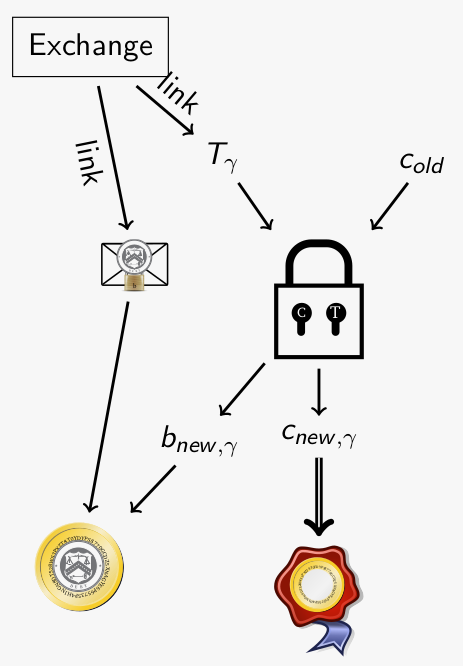
\includegraphics[height=0.5\textwidth]{taler_refresh_link_threat.png}
        \caption{Taler refresh protocol, linkability (source: \cite{pic:refresh-prot})}
        \label{fig:taler-link-threat}
    \end{figure}
    The goal of the cut and choose protocol is to ensure with a high probability ($1/n$) that the customer honestly created the new coin.
    It ensures that the old coin is linked to the new coin via the DH lock.

    With that, the following attack scenario is prevented (with probability $1/n$):\\
    An third party creates the new coin without the DH lock as described in section \ref{sec:blind-sign-schemes}.
    The third party sends the blinded new coin to the customer (who possesses the old coin).
    The customer then signs the new coin by the exchange and sends the blinded signature back to the third party.
    The third party would then be in possession of a valid new coin, which is not linked to the old coin.
    As mentioned, such an attack is detected with a high probability by the exchange with the cut and choose protocol described earlier.

    We will now consider the following attack scenario:\\
    Someone could give the private key of the old coin $c_{old}$ to another person.
    This other person then can derive a new coin using the refresh protocol.
    The original customer currently can not recreate the new coin with only the knowledge of the old coins private key $c_{old}$.
    He would need to know the public key of the transfer key $T_x$ and also the blinded signature of the new coin $f'_{new}$.
    For this reason the exchange exposes the public transfer key $T_x$ and the blinded new coin $f'_{new}$ for a given old coin $C_{old}$.
    So anybody who knows the public key of the old coin could ask for the public transfer key and the blinded signature of the new coin.
    Only a person in possession of the old coins private key $c_{old}$ can recreate the new coin's private key. \\
This mechanism can not be abused for money laundering anymore, since the original customer could trick this third person and spend the coin faster.
The linking protocol is described in figure \ref{fig:refresh-link}.

\begin{figure}
    \begin{equation*}
        \resizebox{1.0\textwidth}{!}{$\displaystyle
        \begin{array}{ l c l }
            % preliminaries
            \text{Customer} &  & \text{Exchange}
            \\ \text{knows:} & & \text{knows:}
            \\ \text{coin}_0 = \langle D_{p(0)}, c_s^{(0)}, C_p^{(0)}, \sigma_{C}^{(0)} \rangle
            \\ & \xrightarrow[\rule{2.5cm}{0pt}]{C_{p(0)}} &
            \\ & &  L := \text{LookupLink}(C_{p(0)})
            \\ & &  \textbf{Comment: } \text{LookupLink}(C_p) \mapsto \{\langle \rho_L^{(i)},
            \\ & & \sigma_L^{(i)}, \overline{\sigma}_C^{(i)} \rangle\}
            \\ & \xleftarrow[\rule{2.5cm}{0pt}]{L} &
            \\ \pcfor \langle \rho_{L}^{(i)}, \overline{\sigma}_L^{(i)}, \sigma_C^{(i)} \rangle \in L
            \\ \langle \hat{C}_p^{(i)}, D_{p(t)}^{(i)}, T_\gamma^{(i)}, \overline{m}_\gamma^{(i)} \rangle := \rho_L^{(i)}
            \\ \langle e_t^{(i)}, N_t^{(i)} \rangle := D_{p(t)}^{(i)}
            \\ \textbf{check } \hat{C}_p^{(i)} \equiv  C_p^{(0)}
            \\ \textbf{check } \text{Ed25519.Verify}(C_p^{(0)}, \rho_{L}^{(i)}, \sigma_L^{(i)})
            \\ x_i := \text{ECDH}(c_s^{(0)}, T_{\gamma}^{(i)})
            \\ r_i := \text{SelectSeeded}(x_i,\mathbb{Z}^*_{N_t})
            \\ c_s^{(i)} := \text{HKDF}(256,x_i,"c")
            \\ C_p^{(i)} := \text{Ed25519.GetPub}(c_s^{(i)})
            \\ \sigma_C^{(i)} := (r_i)^{-1} \cdot \overline{m}_\gamma^{(i)}
            \\ \textbf{check } (\sigma_C^{(i)})^{e_t^{(i)}} \equiv_{N_t^{(i)}} C_p^{(i)}
            \\ \text{(Re-)obtain coin} \langle D_{p(t)}^{(i)},c_s^{(i)}, C_p^{(i)}, \sigma_C^{(i)} \rangle
        \end{array}$
        }
    \end{equation*}
    \caption{Linking protocol}
    \label{fig:refresh-link}
\end{figure}


\subsection{Tipping Protocol}
\label{sec:tipping}
Source for this protocol was section 4.1.10 from \cite{dold:the-gnu-taler-system}.\\
Merchants can give customers a small tip by using the withdraw loophole (described in section \ref{sec:withdraw-loophole}).
This can be for a variety of different reasons, for example for submitting a survey.
The merchant needs to create a reserve with the exchange.
The reserve keys is now used to sign blinded coins generated by the user.
\begin{enumerate}
    \item The Merchant triggers the Payment required response with the Taler-Tip header set
    \item The taler tip header contains information like amount, exchange to use, deadline and more. (details section 4.1.10 \cite{dold:the-gnu-taler-system})
    \item The customer creates planchets that sum up the amount and blinds the token with the denomination key of the specified exchange and sends the blinded planchets to the merchant.
    \item The merchant creates withdrawal confirmations (by signing them with the reserver private key) for these planchets and responds with a list of signatures.
    \item The customer then uses these signatures to create coins as in the withdrawal protocol
\end{enumerate}
The received coins are still anonymized and only spendable by the customer.


\subsection{Refund Protocol}
A merchant can undo a deposit on a coin by signing a refund permission.
The protocol details can be found in section 4.7.5 of \cite{dold:the-gnu-taler-system}.
Since a refund is mainly done by the merchant, to provide refunds a merchant need to support refunds.
A refund can be either fully or partially.
After a refund, the customer is able to spend the coin, but it should be refreshed first to prevent linking of transactions.
The refund deadline is specified in the contract header, after the deadline the exchange makes a wire transfer with the money to the merchants bank.
There is a refund fee, which is subtracted from the remaining coin value.
This also prevents denial of service attacks, or at least makes them economically uninteresting.
There exists automatic refunds when a payment only partially succeeds for many reasons.
Refunds are also an important business case for many merchants who want to provide a convenient experience.
A merchant can for example provide a refund when the customer is not happy with the product.
Such a refund can be made by the merchant with a signature without the customers consent.
Now should be clear what the purpose of a refund protocol is, the rest of this section will look at the refund protocol.


In the protocol the customer requests a refund from the merchant.
If the merchant accepts the request, it authorizes the exchange to apply the refund.
\begin{enumerate}
    \item The customer asks for a refund for payment $p$ with reason $m$
    \item The merchant decides whether it accepts the refund or not according to the merchants business rules.
    \item If accepted, the merchant signs the refund permission with the merchants Ed25519 key and sends it to exchange.
    \item The exchange checks the signature and refunds the coin(s) and sends a signed confirmation to the merchant.
    \item The merchant sends the signed confirmation from the exchange to the customer.
\end{enumerate}

\section{Trust and PKI in Taler}
In this section Taler's \ac{PKI} is explained and how Taler handles trust.
This section is included due to the reason that we have to create Schnorr denomination keys to add the Clause Blind Schnorr Signature scheme to Taler.
Taler uses TLS, however it does not rely on TLS for authenticity or integrity. (More detailed in chapter 4.1.3 of \cite{dold:the-gnu-taler-system})

\subsubsection{Auditor}
In Taler the auditors serves as trust anchor, and they are identified by a single Ed25519 public key.
Similar to the list of trusted root \ac{CA} that come with web browsers and operating systems, a wallet comes with a list of trusted auditor certificates.
In the rest of this section, different parts of Taler and how they are integrated in Taler's \ac{PKI} are discussed.
The section ends with a discussion about security risks of Taler's trust model.
For details, refer to chapter 4.1.3 of \cite{dold:the-gnu-taler-system}.

\begin{figure}[htp]
    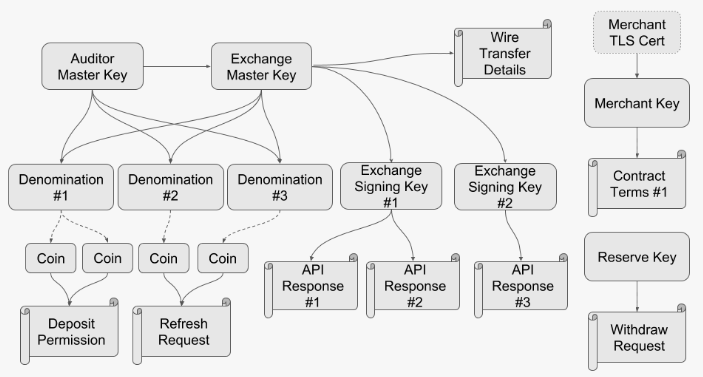
\includegraphics[height=0.5\textwidth]{taler-pki.png}
    \centering
    \caption{GNU Taler PKI entities (source: \cite{dold:the-gnu-taler-system})}
    \label{fig:taler-pki}
\end{figure}

\subsubsection{Exchange}
The exchange has to expose an API in order to enable customers (wallets), merchants and auditors to access keys and other information.
An exchange has a long term master key (Ed25519 key) and a base URL.
The URL and the long term \ac{MK} identifies an exchange.
The \ac{MK} is only used as an offline signing key and should be stored on an air-gapped machine.
Further, the exchange has online signing keys (Ed25519 key), which are signed by the exchanges \ac{MK}.
This \ac{MK} is on his side signed by one or possibly more auditors master key(s).
The exchange's (online) signing keys are used to sign API responses.
The denomination keys of an exchange are also signed by the exchanges offline \ac{MK} and the auditors \ac{MK}.
The bank accounts supported by the exchange for withdrawals and deposits are also signed by the exchanges offline \ac{MK}.

API requests are made to the base URL appending the name of the endpoint (eg. <base-url>/keys)
The endpoint <base-url>/keys is used to get the exchanges signing keys and other information.
Similar to the \ac{CA} trust model, the client (customer or merchant) can validate the signature of the keys, with the list of trusted auditor certs.

\subsubsection{Coins}
As seen in the withdrawal protocol blind signatures are done with RSA public keys (section \ref{sec:blind-rsa-sign}).
These keys are called denomination keys and they represent the coin value of the signed coins.
The following information concerning the denomination keys are signed by the exchanges master key (citation from \cite{dold:the-gnu-taler-system} chapter 4.1.3):
\begin{itemize}
    \item The RSA public key
    \item The start date, after which coins of this denomination can be withdrawn and deposited.
    \item The  withdraw  expiration  date,  after  which  coins  cannot  be  withdrawn anymore, must be after the start date.
    \item The deposit expiration date, after which coins cannot be deposited anymore, must be after the withdraw expiration date.
    \item The legal expiration date, after which the exchange can delete all records about operations with coins of this denominations, must be (typically quite a long time!) after the deposit expiration date.
    \item The fees for a withdraw, deposit, refresh and refund operation with this coin, respectively.
\end{itemize}

As mentioned, the denomination keys are signed by the exchanges \ac{MK} and also by the auditor.

\subsubsection{Merchant}
The merchant has one Ed25519 public key.
With that key the merchant authenticates to the exchange and signs responses to the customer.
Depending on the jurisdiction, an exchange needs to comply to \ac{KYC} regulations.
A merchant which accepts payments from all exchanges (audited by a trusted auditor) therefore needs to fulfill \ac{KYC} registration for all accepted exchange separately.
This is needed to be legally compliant. \\
Like the customer, also the merchant is configured with a set of trusted auditors and exchanges.
A merchant only accepts payments with coins of denominations from a trusted exchange which is audited by a trusted auditor.

For this reason Taler separates this service into an isolated service, similar to on-premise or external payment gateways, which are used by most e-commerce shops nowadays.

\subsubsection{Customer}
A customer has private keys of reserves that they own to authenticate with the exchange.
The public key was communicated to the exchange with the wire transfer. (A bank however is not part of Taler's \ac{PKI}.)
A customer is therefore not registered with an exchange.

Further a customer possesses the private keys of his coins and stores them in a digital wallet.
\subsubsection{Security Discussion}
Taler's trust model is technically similar to the \ac{CA} trust model we know from TLS certificates.
The trust anchor lies with the auditors, whose certificates are pre-configured by the merchant or customer respectively.
However, trust is always somehow attackable.
That does not mean that there is a security issue in the trust model.
When the list of trusted auditor certs of a customer/merchant somehow can be manipulated, the trust model breaks for this entity. \\
One attack scenario would be to attack customers/merchants with a supply-chain attack on the wallets or merchant backends' implementation.
With software supply-chain attacks on the rise in 2020/21 (although the concept is not new) such an attack could have a big impact. \\
Since auditor certs are coupled with the wallet (or merchant) implementation, a bank, country, central bank or auditor will most likely publish a wallet and a merchant implementation for the corresponding Taler ecosystem.
%This would make it possible for the publisher to make changes on the Taler protocol for this specific implementation.
